\documentclass[12pt]{article}

\usepackage[top=3cm,bottom=3cm]{geometry}
\geometry{a4paper}

\usepackage{polyglossia}
\setdefaultlanguage{french}
\usepackage{csquotes}
\usepackage{unicode-math}
%\usepackage{fontspec}
\usepackage{xltxtra}
\usepackage{amsmath}
%\setmathfont{texgyretermes-math.otf}
\setmainfont[Ligatures=Rare]{Linux Libertine O}%

\renewcommand{\textsc}{}

\usepackage[htt]{hyphenat}
\usepackage{subcaption}

\usepackage{amsopn}
\usepackage{stmaryrd} %% llbracket
\usepackage{algorithm2e}

\usepackage{float}

\newenvironment{algorithme}[1][t]
  {\renewcommand{\algorithmcfname}{Algorithme}% Update algorithm name
   \begin{algorithm}[#1]%
  }{\end{algorithm}}


% Macros
\usepackage{xparse}
\usepackage{xifthen} % \ifthenelse

\newtheorem{theorem}{Théorème}[section]
\newtheorem{definit}{Définition}[section]
\newtheorem{corollary}{Corollaire}[theorem]
\newtheorem{lemma}[theorem]{Lemme}

\usepackage{tabularx}
\newcolumntype{Y}{>{\centering\arraybackslash}X}
\usepackage{multirow}


%%%% Imiter Mlapafr2 avec Bibtex %%%%
%% TODO: éliminer les attributs superflus pour la bibliographie
\usepackage[backend=biber,style=authoryear-comp,uniquename=init,firstinits=true,
            %% "et al" pour > deux auteurs, & pour exactement 2
            uniquelist=false,maxcitenames=2,mincitenames=1,maxbibnames=99,
            isbn=false,url=false,doi=false
]{biblatex}

\DeclareSourcemap{
  \maps[datatype=bibtex]{
    \map{
      \step[fieldsource=series,
        match={\regexp{\s}}, replace={\regexp{\\nobreakspace\x20}}]
      }
  }
}

\renewcommand{\cite}{\parencite}
\renewcommand*{\nameyeardelim}{\addcomma \addnbspace}
% \renewcommand*{\multinamedelim}{\space} % fait le contraire de ce qu'on veut
\renewcommand*{\revsdnamedelim}{}
\renewcommand*\finalnamedelim{ \& }

\DefineBibliographyExtras{french}{\restorecommand\mkbibnamelast}

\DeclareNameAlias{default}{last-first}
\DeclareNameAlias{sortname}{last-first}

% Supprimer les guillemets dans les titres
\DeclareFieldFormat[article,incollection,unpublished,inproceedings]{title}{#1}

% Je n'aime pas, mais j'ai l'impression que mlapafr utilise ça
\renewbibmacro{in:}{\printtext{In} \addspace}


% Espaces insécables dans les citations et la bibliographie (noms de
% conférences) ?

\usepackage{xpatch}
\usepackage{xstring}
%\xpatchbibmacro{series+number}{\addspace}{\addnbspace}{}{}

\renewbibmacro*{series+number}{%
  \setunit*{\addnbspace}%
  \printfield{series}%
  \printfield{number}%
  \newunit}


\xpatchbibmacro{textcite}{\addcoma}{}{}{}

\addbibresource{references.bib}

\usepackage{hyperref}
\usepackage{xspace} % Espaces après macros


\usepackage{todonotes}
\newcommand{\question}[1]{\todo[color=green!40]{#1}}
\newcommand{\questioni}[1]{\todo[color=green!40,inline]{#1}}


%%%% Macros Arthur %%%%
\newcommand{\diff}[2]{\frac{\partial{}{#1}}{\partial{}{#2}}}

\usepackage{mathtools}
\DeclarePairedDelimiterX\setc[2]{\{}{\}}{#1 \;\delimsize\vert\; #2}

\newcommand\mimic{\texttt{MIMIC-III} }
\newcommand\wordtovec{\texttt{Word2Vec} }
\newcommand\doctovec{\texttt{Doc2Vec} }
\newcommand\wordpieces{\emph{word pieces} }
\newcommand\bow{\emph{bag of words} }
\newcommand\skipgram{\emph{skip-gram} }
\newcommand\cbow{\emph{CBOW} }
\newcommand\batchnorm{\emph{batch normalization} }
\newcommand\bert{\emph{BERT} }

\newcommand{\contrainte}[1]{($\text{C}_{#1}$)}


% Notation suites mathématiques
%% 3 options - nécessite xparse !
%% \newcommand{\nsuite}[3][i][N]{({#3}_{#1})_{#1=1}^{#2}}
\DeclareDocumentCommand{\nsuite}{ O{N} O{i} m }
  {({#3}_{#2})_{#2=1}^{#1}}

% Notation pour 'la matrice X sans la colonne j'
\newcommand{\matremov}[2]{%
  %%Substitution i et j !
  \StrSubstitute{#2}{j}{\jmath}[\temp]%
  \StrSubstitute{\temp}{i}{\imath}[\tempp]%
  #1_{\hat{\tempp}
  }
}

% Cardinal
\newcommand{\card}[1]{\left\vert{#1}\right\vert}

% Intervalles
\NewDocumentCommand{\INTERVALINNARDS}{ m m }{
    #1 {,} #2
}
\NewDocumentCommand{\inter}{ s m >{\SplitArgument{1}{,}}m m o }{
    \IfBooleanTF{#1}{
        \left#2 \INTERVALINNARDS #3 \right#4
    }{
        \IfValueTF{#5}{
            #5{#2} \INTERVALINNARDS #3 #5{#4}
        }{
            #2 \INTERVALINNARDS #3 #4
        }
    }
}

%% intervalle entier
\newcommand{\ninter}[2]{\llbracket #1...#2 \rrbracket}

% Transposée

\makeatletter
\newcommand*{\transpose}{%
  {\mathpalette\@transpose{}}%
}
\newcommand*{\@transpose}[2]{%
  % #1: math style
  % #2: unused
  \raisebox{0.2em}{$\m@th#1\intercal$}%
}
\makeatother

%% FIXME : pas tout à fait la bonne notation
%% Voir ISO 80000-2 §2-15.7
%% \newcommand*{\tran}{^{\mkern-1.5mu\mathsf{T}}} ?
\newcommand{\tr}[1]{ {#1}^{\! \transpose}}

% Gras
% Précaution pour les lettres avec exposant : voir mathspec !
% FIXME : le " fait buguer \emph ???
\newcommand{\mb}[1]{{\boldsymbol{\mathbf{#1}}}}

% Distance à base de norme

\newcommand*{\newvarcmd}[2]{%
  \newcommand*{#1}[2][]{%
    \begingroup % \sizel and \sizer are local:
      \let\varl\left
      \let\varr\right
      \ifthenelse{\isempty{##1}}{%
        \let\sizel\relax
        \let\sizer\relax
      }{%
        \expandafter\let\expandafter\sizel\csname ##1l\endcsname
        \expandafter\let\expandafter\sizer\csname ##1r\endcsname
      }%
      #2%
    \endgroup
  }
}

\newvarcmd{\abs}{\sizel\lvert #2\sizer\rvert}
\newvarcmd{\norm}{\sizel\lVert #2\sizer\rVert}
\newcommand{\dist}[2]{\norm{#1 - #2}}

%% Macro pour les vecteurs directeurs
\NewDocumentCommand{\vdir}{ m O{j} O{r} }{\mb{#1}_{#3#2}}
\newvarcmd{\primabs}{\sizel\lvert #2\sizer\rvert}

\renewcommand{\eqref}[1]{équation~\ref{#1}}
\newcommand{\algref}[1]{algorithme~\ref{#1}}
\newcommand{\figref}[1]{figure~\ref{#1}}
\newcommand{\tabref}[1]{tableau~\ref{#1}}
\newcommand{\secref}[1]{section~\ref{#1}}

\AtBeginDocument{ %Bizarrerie unicode-math
  \DeclareMathOperator{\mmin}{\mathrm{min}}
  \DeclareMathOperator{\mmax}{\mathrm{max}}
  \DeclareMathOperator{\eexp}{\mathrm{exp}}
  \DeclareMathOperator{\argmin}{\text{argmin}}
  \newcommand{\gargmin}[2]{\argmin_{#1}\left\{{#2}\right\} }
  \DeclareMathOperator{\prox}{\mathrm{prox}}
  \newcommand{\proxg}[3]{\prox_{\frac{#1}{#2}{#3}}}
}

\begin{document}
\title{REDS - TP1 : Analyse préliminaire des données}
\author{Laura Nguyen et Keyvan Beroukhim}
\maketitle

La base de données issue du \emph{ATLAS Higgs Boson Machine Learning Challenge
2014} est constituée de 818238 évènements simulés pouvant être soit des
collisions \emph{"Higgs to tautau"}, soit du \emph{background}. Étant données
ces deux classes, \emph{"s"} pour \emph{signal} et \emph{"b"} pour
\emph{background}, l'objectif est de classifier au mieux les évènements.

\begin{figure}[H]
    \center 
    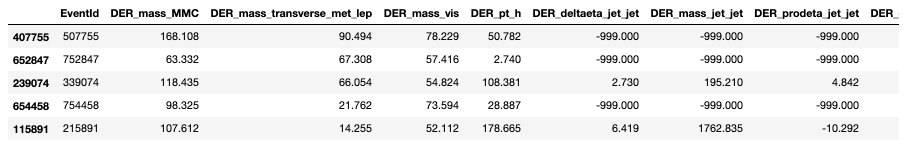
\includegraphics[width=\textwidth]{images/dataset_sample.png}
    \caption{Échantillon de 5 évènements du dataset avec uniquement les 8
    premiers attributs affichés}
\end{figure}

Chaque évènement est défini par 35 attributs, dont son label. Nous retirons du
dataset les features servant uniquement pour le challenge Kaggle :
\texttt{Weight}, \texttt{KaggleSet} et \texttt{KaggleWeight}.

Les données sont composées à 34\% de signaux et à 66\% de background. Nous
remarquons cependant que le dataset contient, à vue d'œil, un nombre important
d'exemples avec des valeurs manquantes (indiquées par -999). Or, travailler avec
des datasets contenant des données manquantes est compliqué. Nous décidons donc
de supprimer les évènements dont au moins un attribut n'est pas valide et nous
nous retrouvons avec seulement 223574 exemples : restreindre le dataset aux
données complètes fait perdre 75\% des données. De plus, la base restreinte
contient 47\% de signaux, soit 13\% de plus que dans le dataset original. Si ce
dernier est représentatif de la réalité alors celui restreint ne l'est pas.


\begin{figure}[H]
    \center
    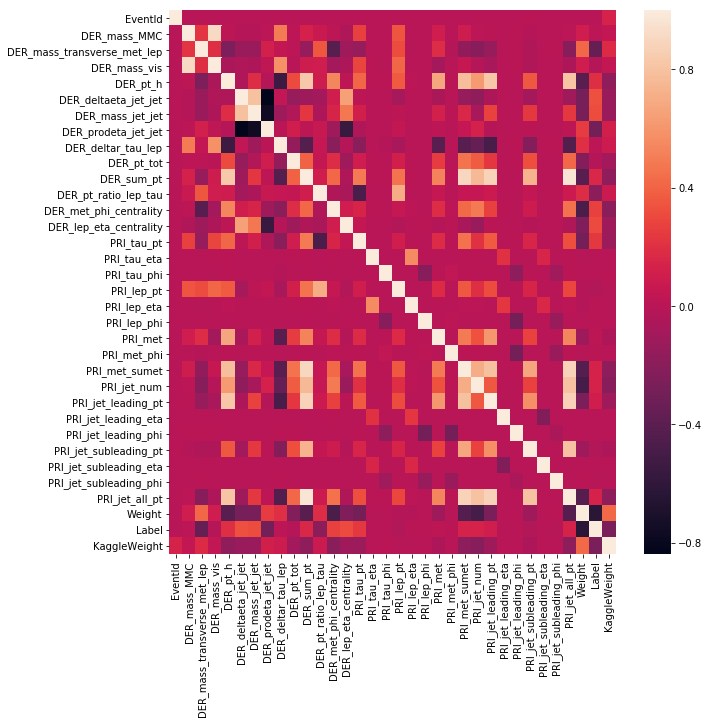
\includegraphics[width=\textwidth]{images/heatmap.png}
    \caption{Matrice de corrélation des attributs en ignorant les valeurs invalides}
    \label{img:heatmap}
\end{figure}

La variable \texttt{EventId} ne fournit pas d'information : cela se remarque,
par exemple, par une corrélation nulle avec toutes les autres variables. Par la
suite, nous ne considérerons donc pas cette variable.


Certaines variables sont fortement corrélées, d'autres anti-corrélées, e.g.
\texttt{DER\_mass\_MMC} et \texttt{DER\_mass\_transverse\_met\_lep}. Ces
informations pourront se révéler utiles si nous souhaitons traiter les évènements à
données manquantes.

La matrice de corrélation obtenue en ignorant les valeurs invalides
et celle obtenue en ignorant les évènements ayant au moins un attribut à valeur
invalide sont très similaires.

\begin{figure}[H]
    \center
    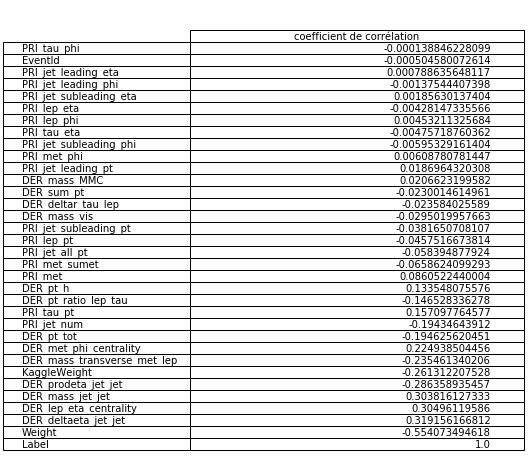
\includegraphics[width=\textwidth]{images/table_corr.png}
    \caption{Coefficients de corrélation entre chaque attribut et la classe
    \texttt{Label}}
    \label{img:table-corr}
\end{figure}

\begin{figure}[H]
    \center 
    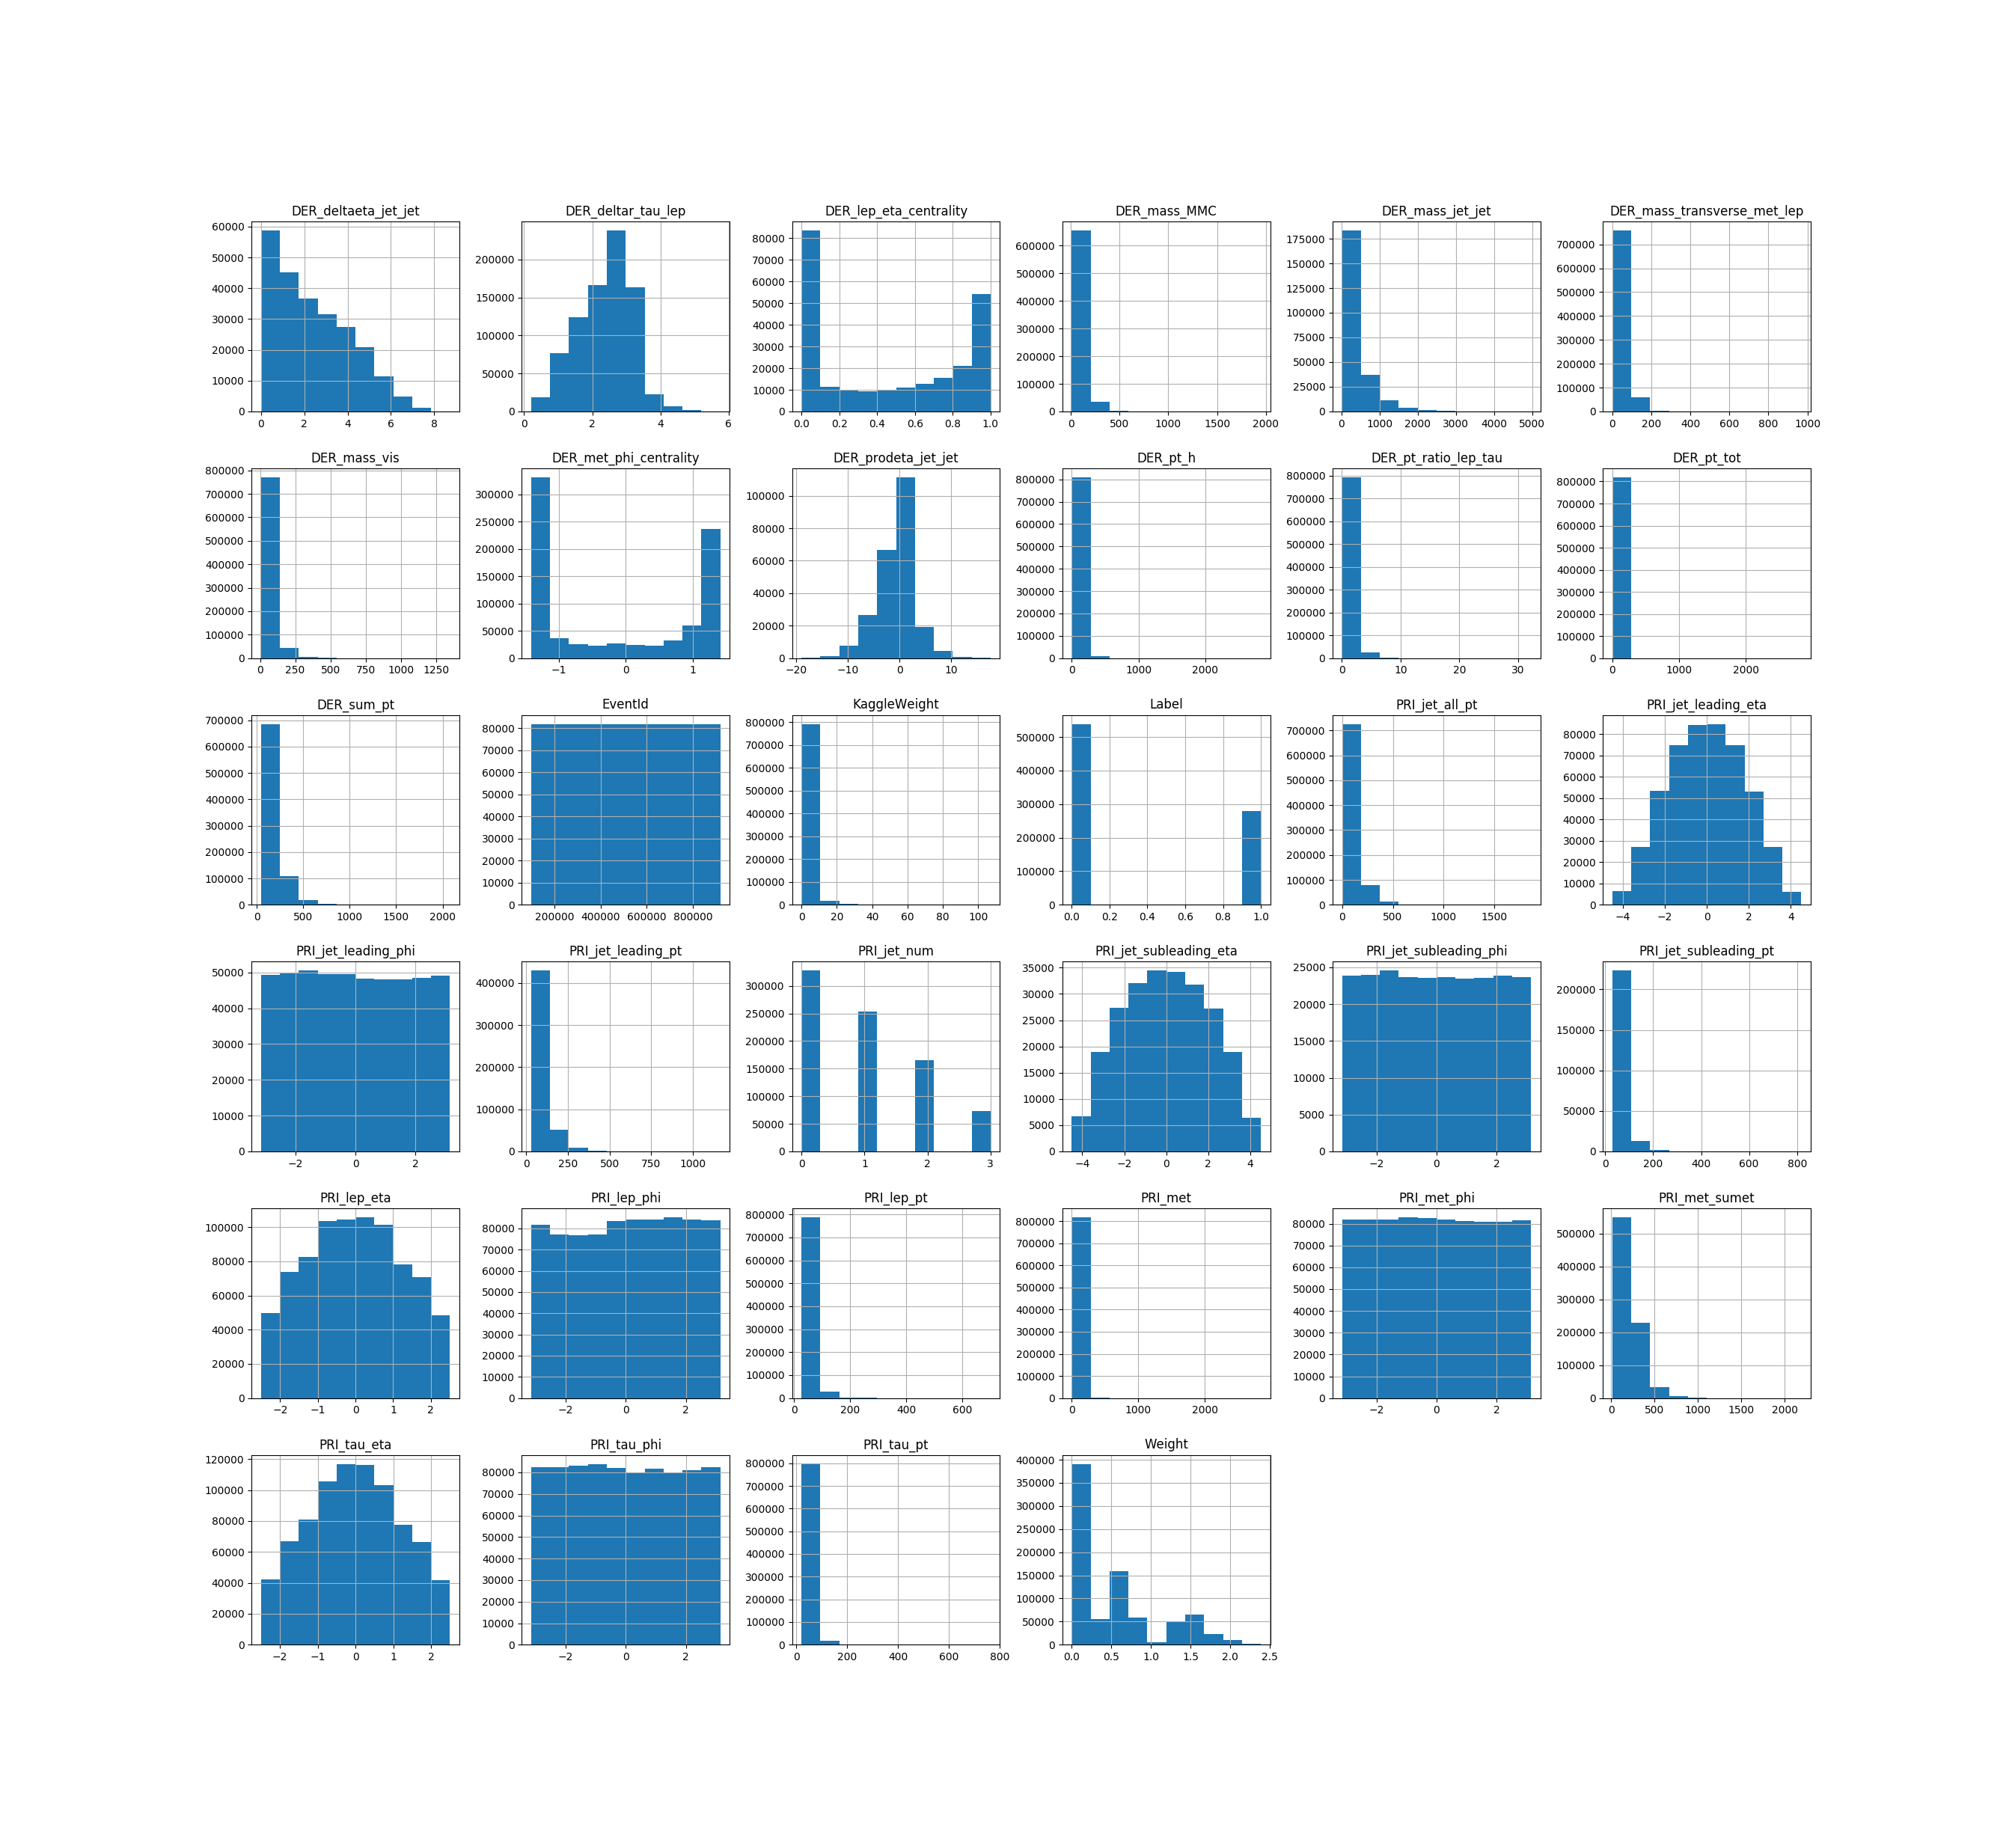
\includegraphics[width=\textwidth]{images/histogrammes.png}
    \caption{Histogramme des valeurs de chaque attribut du dataset où les
    valeurs manquantes sont ignorées}
    \label{img:hist}
\end{figure}

Plusieurs histogrammes sont très déséquilibrés, cela est peut-être dû à une présence d'erreur dans les
données. Nous pourrions essayer de traiter ces cas-là en les supprimant par exemple.

De nombreux histogrammes présentent une répartition exponentielle décroissante des données.

Preprocessing : transformation (non linéaire) de certaines variables en les remplaçant par leur log

%\todo[inline,color=green!40]{(Idée) On pourrait s'aider de la p-value pour
%sélectionner les features
%(https://towardsdatascience.com/feature-selection-correlation-and-p-value-da8921bfb3cf)}

%\section{Semaine du 3 juin}
%
%\begin{itemize}
%    \item Bibliographie : lecture d'articles de recherche
%        \begin{itemize}
%            \item Représentation de documents : \fullcite{le-doc2vec}
%            \item Représentation de mots contextualisée : \fullcite{peters-elmo}
%            \item Représentation de patients : \fullcite{nguyen-deepr}
%        \end{itemize}
%    \item Formation pour avoir accès aux données \mimic 
%        \cite{johnson-mimic}
%    \item Intégration des données \mimic dans une base de données PostgreSQL
%\end{itemize}
%
%\section{Semaine du 10 juin}
%
%\begin{itemize}
%    \item Bibliographie : 
%        \begin{itemize}
%            \item Représentation de mots : \fullcite{mikolov-word2vec}
%            \item Représentation de concepts médicaux  : 
%                \begin{itemize}
%                    \item \fullcite{choi-multi}
%                    \item \fullcite{choi-medical}
%                \end{itemize}
%            \end{itemize}
%
%        \item Réunion avec les encadrants. Dans un premier temps, représentation
%            des compte-rendus de sortie d'hôpital uniquement. 
%
%            Expérience $0$ : pour chaque compte-rendu, prédiction de la première
%            hiérarchie des diagnostics médicaux ($19$ classes) associés, codés
%            selon la norme \texttt{ICD-9}
%            \footnote{https://www.cepidc.inserm.fr/causes-medicales-de-deces/cim-9}.
%
%            Plusieurs représentations des compte-rendus :
%
%            \begin{itemize}
%                \item Bag of Words
%                \item Aggrégation de représentations \wordtovec (\cite{gensim})
%                \item \doctovec
%                \item par réseaux de neurones à attention.
%            \end{itemize}
%
%        \item Prise en main des données \mimic. Analyse des tables : 
%            \begin{itemize}
%                \item \texttt{ADMISSIONS} : données relatives à l'entrée d'un
%                    patient à l'hôpital
%                \item \texttt{NOTEEVENTS} : contient les différents rapports
%                    associés à chaque séjour
%                \item \texttt{DIAGNOSES\_ICD} : diagnostics de chaque patient
%                    pour chaque séjour
%            \end{itemize}
%
%        \item Début de la mise en place d'une baseline : représentation en sac de mots et
%            optimisation d'un SVM linéaire.
%
%            \begin{itemize}
%                \item Pré-traitements du texte : concaténation des rapports de
%                    sortie pour chaque séjour s'il y en a plusieurs, suppression
%                    des balises d'anonymisation
%                \item Développement des outils nécessaires pour vectoriser les
%                    rapports en utilisant la librairie \texttt{scikit-learn}
%                    \cite{scikit}
%                \item Construction de représentations BoW des
%                    documents selon différentes combinaisons de pré-traitements
%                \begin{enumerate}
%                    \item Pas de pré-traitement
%                    \item Suppression des stopwords
%                    \item Suppression des stopwords, stemmatisation
%                    \item Suppression des stopwords, des nombres,
%                        stemmatisation, mise en minuscules des lettres
%                    \item Suppression des stopwords, des nombres,
%                        stemmatisation, mise en minuscules des lettres, seuil
%                        sur la fréquence maximale d'apparition dans les
%                        documents
%                    \item Bigrammes, pas de pré-traitement
%                    \item Bigrammes, suppression des stopwords
%                    \item Bigrammes, suppression des stopwords, stemmatisation
%                    \item Bigrammes, suppression des stopwords, des nombres,
%                        stemmatisation, mise en minuscules des lettres
%                    \item Bigrammes, suppression des stopwords, des nombres,
%                        stemmatisation, mise en minuscules des lettres, seuil
%                        sur la fréquence maximale d'apparition dans les
%                        documents
%                \end{enumerate}
%            \end{itemize}
%\end{itemize}
%
%\section{Semaine du 17 juin}
%
%\begin{itemize}
%    \item Fin de la mise en place de la baseline : évaluation des différentes
%        représentations de compte-rendus
%        \begin{itemize}
%            \item Modification des objets à représenter : représentation de
%                chaque rapport pris individuellement, la concaténation rendant
%                les documents trop longs et donc le temps de calcul trop
%                important
%            \item Classification multi-classes multi-labels : pour chaque
%                représentation des documents, méthode one against all à base de
%                SVM linéaire et optimisation de $C$ par validation croisée
%
%            \item Résultats :
%
%                \begin{table}[H]
%                \centering
%                \resizebox{\textwidth}{!}{
%                \begin{tabular}{c|c|c|c|c}
%                        Version & Précision pondérée & Rappel pondéré & F1
%                        pondéré & Hamming \\
%                        \hline
%                        1 & 0.701  & 0.715 & 0.705 & 0.531\\
%                        2 & 0.704 & 0.716 & 0.706 & 0.532 \\
%                        3 & 0.712 & 0.720 & 0.712 & 0.541 \\
%                        4 &  0.713 & 0.724 & 0.714 & 0.542 \\
%                        5 & 0.710 & 0.732 & 0.716 & 0.545 \\
%                        6 & 0.687 & 0.698 & 0.691 & 0.518 \\
%                        7 & 0.678 & 0.698 & 0.685 & 0.507 \\
%                        8 & 0.689 & 0.701 & 0.693 & 0.517 \\
%                        9 & 0.737 & 0.661 & 0.645 & 0.551 \\
%                        10 & 0.681 & 0.717 & 0.695 & 0.516 \\
%                \end{tabular}}
%                \caption{Scores obtenus pour chaque représentation \bow des
%                    compte-rendus}
%                \end{table}
%        \end{itemize}
%    \item Représentation des compte-rendus par aggrégation de vecteurs de mots
%        construits avec l'implémentation \texttt{gensim} \cite{gensim} de
%        \wordtovec \cite{mikolov-word2vec}
%
%        \begin{itemize}
%            \item Entraînement d'un modèle à partir des compte-rendus uniquement 
%                \begin{itemize}
%                    \item Similarité entre "great" et "good" : 0.18673581
%                    \item Similarité entre "great" et "bad" : 0.12311481
%                    \item 
%                    \begin{figure}[H]
%                	    \center 
%                	    \includegraphics[width=0.8\textwidth]{images/word2vec/sim-v0.png}
%                    \end{figure}
%                \end{itemize}
%            \item Utilisation de vecteurs de mots pré-entraînés sur un corpus
%                Wikipedia \cite{pennington-glove}
%                
%                \begin{itemize}
%                    \item Similarité entre "great" et "good" : 0.64100474
%                    \item Similarité entre "great" et "bad" : 0.34945
%                \end{itemize}
%
%            \item Entraînement d'un modèle à partir de vecteurs de mots
%                pré-entraînés sur le corpus Wikipedia sus-mentionné
%
%                \begin{itemize}
%                    \item Similarité entre "great" et "good" : 0.6481616 
%                    \item Similarité entre "great" et "bad" : 0.36196503 
%                    \item 
%                    \begin{figure}[H]
%                	    \center 
%                	    \includegraphics[width=0.8\textwidth]{images/word2vec/sim-v1.png}
%                    \end{figure}
%                \end{itemize}
%
%            \item Utilisation de vecteurs de mots pré-entraînés sur un corpus
%                de données biomédicales \cite{mcdonald-deep}
%                
%                \begin{itemize}
%                    \item Similarité entre "great" et "good" : 0.45916468
%                    \item Similarité entre "great" et "bad" : 0.2333424
%                \end{itemize}
%
%            \item Entraînement d'un modèle à partir de vecteurs de mots
%                pré-entraînés sur le corpus de données bio-médicales sus-mentionné
%
%                \begin{itemize}
%                    \item Similarité entre "great" et "good" : 0.45916468
%                    \item Similarité entre "great" et "bad" : 0.2333424
%                    \item 
%                    \begin{figure}[H]
%                	    \center 
%                	    \includegraphics[width=0.8\textwidth]{images/word2vec/sim-v2.png}
%                    \end{figure}
%                \end{itemize}
%
%                
%        \end{itemize}
%\end{itemize}
%
%\section{Semaine du 24 juin}
%
%\begin{itemize}
%    \item Re-modification des objets à représenter : concaténation des rapports
%        de sortie pour chaque séjour s'il y en a plusieurs (la version
%        précédente contenait des erreurs)
%    
%    \item Résultats sur la baseline précédente :
%
%                \begin{table}[H]
%                \centering
%                \resizebox{\textwidth}{!}{
%                \begin{tabular}{c|c|c|c|c}
%                        Version & Précision pondérée & Rappel pondéré & F1
%                        pondéré & Hamming \\
%                        \hline
%                        1 & 0.694  & 0.724 & 0.705 & 0.546\\
%                        2 & 0.695 & 0.723 & 0.705 & 0.545 \\
%                        3 & 0.700 & 0.729 & 0.710 & 0.551 \\
%                        4 &  0.704 & 0.733 & 0.714 & 0.553 \\
%                        5 & 0.699 & 0.744 & 0.716 & 0.554 \\
%                        6 & 0.676 & 0.704 & 0.688 & 0.531 \\
%                        7 & 0.670 & 0.705 & 0.685 & 0.523 \\
%                        8 & 0.682 & 0.710 & 0.693 & 0.533 \\
%                        9 & 0.676 & 0.724 & 0.695 & 0.529 \\
%                        10 & 0.673 & 0.728 & 0.700 & 0.529 \\
%                \end{tabular}}
%                \caption{Scores obtenus pour chaque représentation \bow des
%                    compte-rendus}
%                \end{table}
%
%
%    \item Mise en place d'une seconde baseline :
%        \begin{itemize}
%            \item les compte-rendus (20000 dans un premier temps), d'abord
%                pré-traités (suppression des balises d'anonymisation, des
%                nombres, mise en minuscules) sont représentés par des vecteurs
%                de mots (construits par \wordtovec) moyennés
%            \item le modèle utilisé est un réseau de neurones implémenté sur
%                \texttt{PyTorch} \cite{pytorch} correspondant à une régression
%                logistique, i.e., il comprend une couche linéaire avec autant de
%                sorties que de classes ainsi qu'une activation sigmoïde
%                renvoyant la probabilité d'appartenance d'un exemple à chaque
%                label.
%        \end{itemize}
%
%        On considère plusieurs façons d'entraîner ces vecteurs de mots :
%
%        \begin{enumerate}
%            \item À partir des compte-rendus médicaux uniquement 
%            \item En entraînant un modèle à partir de vecteurs pré-entraînés sur
%                un corpus Wikipedia \cite{pennington-glove}
%            \item En entraînant un modèle à partir de vecteurs pré-entraînés sur
%                des articles bio-médicaux \cite{mcdonald-deep}
%        \end{enumerate}
%
%        Outre la taille des vecteurs (300 pour les deux premiers modèles, 200
%        pour le dernier), on utilise la configuration par défaut de \wordtovec
%        (\figref{img:w2v-defaut}).
%
%        \begin{figure}[H]
%            \center 
%            \includegraphics[width=\textwidth]{images/word2vec/w2v-defaut.png}
%            \caption{Configuration par défaut de \wordtovec}
%            \label{img:w2v-defaut}
%        \end{figure}
%
%        \begin{figure}[H]
%            \center 
%            \includegraphics[width=\textwidth]{images/word2vec/w2v-parameters.png}
%            \caption{Paramètres de \wordtovec}
%            \label{img:w2v-parameters}
%        \end{figure}
%
%        Pour chaque modèle, un réseau de neurones tel que décrit ci-haut est
%        optimisé en utilisant la bibliothèque \texttt{Tune} \cite{tune} du
%        framework \texttt{Ray}. Les hyperparamètres à optimiser sont le
%        \emph{learning rate}, le nombre d'itérations et le momentum. La fonction
%        de coût utilisée est la \emph{binary cross-entropy}.
%
%        Résultats :
%
%            \begin{table}[H]
%            \centering
%            \resizebox{\textwidth}{!}{
%            \begin{tabular}{c|c|c|c|c}
%                    Version & Précision pondérée & Rappel pondéré & F1
%                    pondéré & Hamming \\
%                    \hline
%                    1 & 0.398  & 0.539 & 0.365 & 0.206\\
%                    2 & 0.400 & 0.800 & 0.495 & 0.286 \\
%                    3 & 0.290 & 0.601 & 0.359 & 0.234 \\
%            \end{tabular}}
%            \caption{Scores obtenus pour chaque modèle \wordtovec}
%            \end{table}
%
%\end{itemize}
%
%\section{Semaine du 1er juillet}
%
%\begin{itemize}
%    \item Mise en place d'un CNN pour la classification multi-classes
%        multi-labels. Ce réseau prend en entrée un batch de documents, où chaque
%        document est représenté par un tenseur \textit{dimension de l'espace
%        latent} $\times$ \textit{taille du document le plus long} contenant,
%        pour chaque mot le constituant, l'embedding correspondant. Ce tenseur
%        est préalablement obtenu en appliquant la couche \texttt{Embedding} sur
%        une matrice \textit{nombre de documents} $\times$ \textit{taille du
%        document le plus long} qui comprend les indices de chaque mot
%        constituant chaque document.
%
%        Les hyperparamètres du CNN sont la matrice de poids pour la création de
%        la couche \texttt{Embedding}, le nombre de filtres, la taille du noyau,
%        la dimension de l'espace latent et le nombre de classes. 
%
%        Les couches sont les suivantes :
%        \begin{enumerate}
%            \item \texttt{Conv1d} avec \texttt{in\_channels=embedding\_dim,
%                out\_channels=n\_kernels,kernel\_size=kernel\_size,padding=1}
%            \item \texttt{AdaptiveMaxPool1d} avec \texttt{output\_size = 1}
%            \item \texttt{Linear} avec
%                \texttt{in\_features=n\_kernels,out\_features=n\_labels}
%            \item \texttt{Sigmoid}
%        \end{enumerate}
%    
%        \item En entraînant un modèle \wordtovec uniquement sur le corpus
%            médical et en fixant le nombre de filtres à 400, la taille du noyau à 5,
%            le nombre de couches à 1, le \emph{learning rate} à $10^{-3}$ et
%            le nombre d'itérations à 3, on obtient les résultats suivants :
%
%        \begin{table}[H]
%        \centering
%        \resizebox{\textwidth}{!}{
%        \begin{tabular}{c|c|c|c|c}
%                Représentation & Précision pondérée & Rappel pondéré & F1
%                pondéré & Hamming \\
%                \hline
%                Moyenne & 0.437  & 0.403 & 0.374 & 0.189 \\
%                CNN & 0.289 & 0.568 & 0.343 & 0.218 \\
%        \end{tabular}}
%        \caption{Scores obtenus pour chaque type d'agrégation des
%            représentations}
%        \end{table}
%
%        \begin{table}[H]
%        \centering
%        \resizebox{0.3\textwidth}{!}{
%            \begin{tabular}{c|c|c}
%                Classe & Moyenne & CNN \\
%                \hline
%                1 & 15.48\% & 100\% \\ 
%                2 & 8.47\% & 0\% \\ 
%                3 & 42.66\% & 44.44\% \\  
%                4 & 16.17\% & 100\%\\
%                5 & 25.88\% & 100\% \\
%                6 & 3.81\% & 100\% \\
%                7 & 63.29\% & 100\% \\
%                8 & 71.90\% & 0\%\\
%                9 & 97.20\% & 100\% \\
%                10 & 30.45\% & 25.00 \%\\ 
%                11 & 84.21\% & 0\%\\
%                12 & 39.71\% & 100\% \\
%                13 & 39.58\% & 100\%\\ 
%                14 & 90.75\% & 100\%\\
%                15 & 40.80\% & 100\%\\
%                16 & 17.37\% & 0\%\\
%                17 & 13.81\% & 0\%\\
%                18 & 37.40\% & 0\%\\
%                19 & 29.23\% & 0\%\\
%        \end{tabular}}
%        \caption{Pour chaque type d'agrégation des représentations, rappel
%            obtenu pour chaque classe}
%        \end{table}
%
%        \begin{table}[H]
%        \centering
%        \resizebox{0.3\textwidth}{!}{
%            \begin{tabular}{c|c|c}
%                Classe & Moyenne & CNN \\
%                \hline
%                1 & 21.73\% & 7.69\% \\ 
%                2 & 16.28\% & 0\% \\ 
%                3 & 73.58\% & 66.67\% \\  
%                4 & 34.41\% & 50.00\%\\
%                5 & 20.15\% & 12.50\% \\
%                6 & 29.14\% & 12.50\% \\
%                7 & 85.13\% & 68.75\% \\
%                8 & 41.86\% & 0\%\\
%                9 & 34.10\% & 25.00\% \\
%                10 & 34.98\% & 10.00 \%\\ 
%                11 & 0.28\% & 0\%\\
%                12 & 8.15\% & 6.25\% \\
%                13 & 11.16\% & 25.00\%\\ 
%                14 & 6.12\% & 25.00\%\\
%                15 & 8.55\% & 18.75\%\\
%                16 & 22.24\% & 0\%\\
%                17 & 37.99\% & 0\%\\
%                18 & 17.63\% & 0\%\\
%                19 & 59.55\% & 0\%\\
%        \end{tabular}}
%        \caption{Pour chaque type d'agrégation des représentations,
%            précision 
%            obtenue pour chaque classe}
%        \end{table}
%\end{itemize}
%
%\section{Semaines du 8 et du 15 juillet}
%
%    Les vecteurs de mots considérés sont de dimension 300. On considère les
%    modèles \wordtovec suivants :
%
%    \begin{enumerate}
%        \item Un modèle entraîné uniquement sur les compte-rendus médicaux
%        \item Un autre pré-entraîné sur un corpus Wikipedia \cite{pennington-glove}
%        \item Un dernier entraîné seulement sur les compte-rendus médicaux mais
%            où les vecteurs représentent des \wordpieces
%    \end{enumerate}
%
%    Les deux façons d'entraîner les modèles sont :
%
%    \begin{itemize}
%        \item considérer tous les compte-rendus puis utiliser \skipgram (taille du vocabulaire : 43584)
%        \item considérer une partie des compte-rendus (20000) puis utiliser
%            \cbow et le \emph{hierarchical softmax} (taille du vocabulaire : 26352)
%    \end{itemize}
%
%    \subsection{Baselines : régression logistique sur des moyennes de vecteurs
%    d'embeddings}
%
%    \emph{Grid search} pour trouver les valeurs optimales du \emph{learning
%    rate} et du nombre d'itérations afin d'entraîner une régression logistique.
%    Le nombre d'itérations maximal est de 100. On récupère le nombre
%    d'\emph{epochs} qui permet d'obtenir un coût minimal sur les données de
%    validation.
%
%        % old
%        %\begin{figure}[H]
%        %	\centering
%        %    \begin{subfigure}[c]{\textwidth}
%        %        \includegraphics[width=1.2\textwidth]{images/word2vec/baseline1-opt-plots.png}
%        %    \caption{Premier modèle \wordtovec}
%        %    \end{subfigure}
%
%        %    \begin{subfigure}[c]{\textwidth}
%        %        \includegraphics[width=1.2\textwidth]{images/word2vec/baseline2-opt-plots.png}
%        %    \caption{Deuxième modèle \wordtovec}
%        %    \end{subfigure}
%
%        %    \begin{subfigure}[c]{\textwidth}
%        %        \includegraphics[width=1.2\textwidth]{images/word2vec/baseline3-opt-plots.png}
%        %    \caption{Troisième modèle \wordtovec}
%        %    \end{subfigure}
%
%        %    \caption{Coût \emph{Binary cross-entropy} en fonction du pas (bleu : entraînement, rouge : validation)}        
%        %\end{figure}
%
%    \begin{figure}[H]
%    	\centering
%        \begin{subfigure}[c]{\textwidth}
%            \includegraphics[width=1.2\textwidth]{images/word2vec/baseline1-all-opt-plots.png}
%        \caption{Premier modèle \wordtovec}
%        \end{subfigure}
%
%        \begin{subfigure}[c]{\textwidth}
%            \includegraphics[width=1.2\textwidth]{images/word2vec/baseline2-all-opt-plots.png}
%        \caption{Deuxième modèle \wordtovec}
%        \end{subfigure}
%
%        \begin{subfigure}[c]{\textwidth}
%            \includegraphics[width=1.2\textwidth]{images/word2vec/baseline3-all-opt-plots.png}
%        \caption{Troisième modèle \wordtovec}
%        \end{subfigure}
%
%        \caption{Modèles appris sur tous les documents avec \skipgram : coût
%        \emph{Binary cross-entropy} en fonction du pas (bleu : entraînement,
%        rouge : validation) (\skipgram en considérant tous les documents)}        
%    \end{figure}
%
%    \begin{figure}[H]
%    	\centering
%        \begin{subfigure}[c]{\textwidth}
%            \includegraphics[width=1.2\textwidth]{images/word2vec/baseline1-cbow-opt-plots.png}
%        \caption{Premier modèle \wordtovec}
%        \end{subfigure}
%
%        \begin{subfigure}[c]{\textwidth}
%            \includegraphics[width=1.2\textwidth]{images/word2vec/baseline2-cbow-opt-plots.png}
%        \caption{Deuxième modèle \wordtovec}
%        \end{subfigure}
%
%        \begin{subfigure}[c]{\textwidth}
%            \includegraphics[width=1.2\textwidth]{images/word2vec/baseline3-cbow-opt-plots.png}
%        \caption{Troisième modèle \wordtovec}
%        \end{subfigure}
%
%        \caption{Modèles appris sur 20000 documents avec \cbow : coût
%        \emph{Binary cross-entropy} en fonction du pas (bleu : entraînement,
%        rouge : validation) (\cbow en considérant une partie des documents)}        
%    \end{figure}
%
%        % old
%        %\begin{table}[H]
%        %\resizebox{1.1\textwidth}{!}{
%        %    \begin{tabular}{c|*{7}{c|}c}
%        %        \multirow{2}{*}{} & \multicolumn{2}{c|}{Précision pondérée} &
%        %        \multicolumn{2}{c|}{Rappel pondéré} &
%        %        \multicolumn{2}{c|}{F1 pondéré} &
%        %        \multicolumn{2}{c}{Hamming}\\ \cline{2-3} \cline{4-5} \cline{6-7} \cline{7-9}
%        %        & Apprentissage & Test  & Apprentissage & Test & Apprentissage & Test  & Apprentissage & Test \\
%        %        \hline
%        %        1 & 76.95\% & 75.46\% & 64.59\% & 63.71\% & 68.61\% & 67.49\%
%        %        & 57.24\% & 56.39\% \\
%        %        2 & 77.11\% & 75.23\% & 55.24\% & 54.72\% & 60.30\% & 59.64\%
%        %        & 51.09\% & 50.56\% \\
%        %        3 & 72.42\% & 69.39\% & 54.42\% & 53.62\% & 57.45\% & 56.47\%
%        %        & 48.92\% & 48.31\% \\
%        %\end{tabular}}
%        %\caption{Pour chaque modèle \wordtovec, scores obtenus sur les données
%        %    d'apprentissage et de test avec les hyperparamètres optimaux} 
%        %\end{table}
%
%
%        \begin{table}[H]
%        \resizebox{1.1\textwidth}{!}{
%            \begin{tabular}{c|*{7}{c|}c}
%                \multirow{2}{*}{} & \multicolumn{2}{c|}{Précision pondérée} &
%                \multicolumn{2}{c|}{Rappel pondéré} &
%                \multicolumn{2}{c|}{F1 pondéré} &
%                \multicolumn{2}{c}{Hamming}\\ \cline{2-3} \cline{4-5} \cline{6-7} \cline{7-9}
%                & Apprentissage & Test  & Apprentissage & Test & Apprentissage & Test  & Apprentissage & Test \\
%                \hline
%                1 & 77.41\% & 76.36\% & 59.98\% & 59.54\% & 64.65\% & 64.10\%
%                & 54.50\% & 54.11\% \\
%                2 & 75.33\% & 74.14\% & 58.96\% & 58.39\% & 62.48\% & 61.83\%
%                & 52.99\% & 52.59\% \\
%                3 & 74.10\% & 73.59\% & 54.05\% & 53.39\% & 58.09\% & 57.38\%
%                & 49.43\% & 49.07\% \\
%        \end{tabular}}
%        \caption{Pour chaque modèle \wordtovec entraîné sur tous les documents
%            avec \skipgram, scores obtenus sur les données
%            d'apprentissage et de test avec les hyperparamètres optimaux} 
%        \end{table}
%
%        \begin{table}[H]
%        \resizebox{1.1\textwidth}{!}{
%            \begin{tabular}{c|*{7}{c|}c}
%                \multirow{2}{*}{} & \multicolumn{2}{c|}{Précision pondérée} &
%                \multicolumn{2}{c|}{Rappel pondéré} &
%                \multicolumn{2}{c|}{F1 pondéré} &
%                \multicolumn{2}{c}{Hamming}\\ \cline{2-3} \cline{4-5} \cline{6-7} \cline{7-9}
%                & Apprentissage & Test  & Apprentissage & Test & Apprentissage & Test  & Apprentissage & Test \\
%                \hline
%                1 & 78.25\% & 76.74\% & 63.54\% & 62.74\% & 68.53\% & 67.40\%
%                & 57.27\% & 56.43\% \\
%                2 & 74.67\% & 73.13\% & 57.88\% & 57.16\% & 62.01\% & 61.19\%
%                & 52.03\% & 51.46\% \\
%                3 & 74.32\% & 72.47\% & 55.98\% & 55.27\% & 59.85\% & 58.93\%
%                & 50.51\% & 50.08\% \\
%        \end{tabular}}
%        \caption{Pour chaque modèle \wordtovec entraîné sur tous 20000 documents
%            avec \cbow, scores obtenus sur les données
%            d'apprentissage et de test avec les hyperparamètres optimaux} 
%        \end{table}
%        
%        % old
%        %\begin{table}[H]
%        %\resizebox{1.1\textwidth}{!}{
%        %    \begin{tabular}{c|*{7}{c|}c}
%        %        \multirow{2}{*}{} & \multicolumn{2}{c|}{Précision pondérée} &
%        %        \multicolumn{2}{c|}{Rappel pondéré} &
%        %        \multicolumn{2}{c|}{F1 pondéré} &
%        %        \multicolumn{2}{c}{Hamming}\\ \cline{2-3} \cline{4-5} \cline{6-7} \cline{7-9}
%        %        & Apprentissage & Test  & Apprentissage & Test & Apprentissage & Test  & Apprentissage & Test \\
%        %        \hline
%        %        1 & 76.95\% & 75.46\% & 64.59\% & 63.71\% & 68.61\% & 67.49\%
%        %        & 57.24\% & 56.39\% \\
%        %        2 & 77.11\% & 75.23\% & 55.24\% & 54.72\% & 60.30\% & 59.64\%
%        %        & 51.09\% & 50.56\% \\
%        %        3 & 72.42\% & 69.39\% & 54.42\% & 53.62\% & 57.45\% & 56.47\%
%        %        & 48.92\% & 48.31\% \\
%        %\end{tabular}}
%        %\caption{Pour chaque modèle \wordtovec, scores obtenus sur les données
%        %    d'apprentissage et de test avec les hyperparamètres optimaux} 
%        %\end{table}
%
%    \subsection{CNN}
%
%    \emph{Grid search} pour trouver les hyperparamètres optimaux d'une
%        architecture CNN à 1, 2 et 3 couches. Le \emph{learning rate} est fixé à
%        $1e^{-3}$ et le nombre d'itérations à 30. On récupère le nombre
%        d'\emph{epochs} qui permet d'obtenir un coût minimal sur les données de
%        validation. Les valeurs des hyperparamètres sont les suivants :
%    \begin{itemize}
%        \item Terme de pénalité : $1e^{-4}, 1e^{-3}, 1e^{-2}, 1e^{-1},
%            0$
%        \item Taille des filtres :
%            \begin{itemize}
%                \item 1 couche : 3,5
%                \item 2 couches : (3,3), (5,5)
%                \item 3 couches : (3,3,3), (5,5,5)
%            \end{itemize}
%        \item Taille des fenêtres de \emph{max-pooling} :
%            \begin{itemize}
%                \item 2 couches : 2, 3
%                \item 3 couches : (2,2), (3,3)
%            \end{itemize}
%        \item Nombre de filtres :
%            \begin{itemize}
%                \item 1 couche : 10, 50, 100
%                \item 2 couches : (20,20), (50,50), (20,50), (50,20)
%                \item 3 couches : (20,20,20), (50,50,50), (10,20,50), (50,20,10)
%            \end{itemize}
%    \end{itemize}
%
%    \subsubsection{Apprentissage des modèles sur toutes les données avec
%    \skipgram et régularisation L2}
%
%    \begin{enumerate}
%        \item Premier modèle \wordtovec : vecteurs de mots construits uniquement
%            à partir des compte-rendus médicaux
%
%    %\begin{table}[H]
%    %\centering
%    %\resizebox{0.8\textwidth}{!}{
%    %\begin{tabular}{c|c|c|c}
%    %    & 1 couche & 2 couches & 3 couches\\
%    %    \hline
%    %    Nombre d'itérations & 4 & 3 &  4 \\
%    %    Taille des filtres &  3 & (3,3) & (3,3,3) \\
%    %    Taille des fenêtres (\emph{max-pool}) & & 2 &  (2,2) \\
%    %    Nombre de filtres & 100 & (50,50) & (50,50,50)\\
%    %\end{tabular}}
%    %\caption{Paramètres optimaux pour chaque architecture}
%    %\end{table}
%
%    \begin{table}[H]
%    \centering
%    \resizebox{0.8\textwidth}{!}{
%    \begin{tabular}{c|c|c|c}
%        & 1 couche & 2 couches & 3 couches\\
%        \hline
%        Terme de pénalité & $1e^{-4}$ & $1e^{-4}$& $1e^{-4}$\\
%        Nombre d'itérations & 6 & 8 & 10 \\
%        Taille des filtres &  3 & (3,3) & (3,3,3) \\
%        Taille des fenêtres (\emph{max-pool}) & & 2 & (2,2) \\
%        Nombre de filtres & 200 & (100,200) & (50, 100, 200)\\
%    \end{tabular}}
%    \caption{Paramètres optimaux pour chaque architecture}
%    \end{table}
%
%    %\begin{figure}[H]
%    %	\centering
%    %    \begin{subfigure}[c]{\textwidth}
%    %        \includegraphics[width=1.2\textwidth]{images/word2vec/cnn-tuning1-1layer-opt-plots.png}
%
%    %    \caption{1 couche}
%    %    \end{subfigure}
%
%    %    \begin{subfigure}[c]{\textwidth}
%    %        \includegraphics[width=1.2\textwidth]{images/word2vec/cnn-tuning1-2layers-opt-plots.png}
%
%    %    \caption{2 couches}
%    %    \end{subfigure}
%
%    %    \begin{subfigure}[c]{\textwidth}
%    %        \includegraphics[width=1.2\textwidth]{images/word2vec/cnn-tuning1-3layers-opt-plots.png}
%    %    \caption{3 couches}
%    %    \end{subfigure}
%
%    %    \caption{Coût \emph{Binary cross-entropy} en fonction du pas (bleu : entraînement, rouge : validation)}        
%    %\end{figure}
%
%    \begin{figure}[H]
%    	\centering
%        \begin{subfigure}[c]{\textwidth}
%            \includegraphics[width=1.2\textwidth]{images/word2vec/cnn-tuning1-all-1layer-L2-plots.png}
%
%        \caption{1 couche}
%        \end{subfigure}
%
%        \begin{subfigure}[c]{\textwidth}
%            \includegraphics[width=1.2\textwidth]{images/word2vec/cnn-tuning1-all-2layers-L2-plots.png}
%
%        \caption{2 couches}
%        \end{subfigure}
%
%        \begin{subfigure}[c]{\textwidth}
%            \includegraphics[width=1.2\textwidth]{images/word2vec/cnn-tuning1-all-3layers-L2-plots.png}
%        \caption{3 couches}
%        \end{subfigure}
%
%        \caption{Coût \emph{Binary cross-entropy} en fonction du pas (bleu :
%        entraînement, rouge : validation)}        
%    \end{figure}
%
%    %\begin{table}[H]
%    %\resizebox{1.1\textwidth}{!}{
%    %    \begin{tabular}{c|*{7}{c|}c}
%    %        \multirow{2}{*}{} & \multicolumn{2}{c|}{Précision pondérée} &
%    %        \multicolumn{2}{c|}{Rappel pondéré} &
%    %        \multicolumn{2}{c|}{F1 pondéré} &
%    %        \multicolumn{2}{c}{Hamming}\\ \cline{2-3} \cline{4-5} \cline{6-7} \cline{7-9}
%    %        & Apprentissage & Test  & Apprentissage & Test & Apprentissage & Test  & Apprentissage & Test \\
%    %        \hline
%    %        1 couche & 79.78\% & 76.20\% & 67.16\% & 64.55\% & 70.84\% & 67.80\%
%    %        & 60.30\% & 57.32\% \\
%    %        2 couches & 73.16\% & 70.61\% & 69.17\% & 67.29\% & 69.76\% & 67.72\%
%    %        & 58.06\% & 56.25\% \\
%    %        3 couches & 76.27\% & 77.35\% & 60.21\% & 59.09\% & 63.97\% & 62.61\%
%    %        & 55.34\% & 54.38\% \\
%    %\end{tabular}}
%    %\caption{Scores obtenus sur les données d'apprentissage et de test avec
%    %        les hyperparamètres optimaux} 
%    %\end{table}
%
%    \begin{table}[H]
%    \resizebox{1.1\textwidth}{!}{
%        \begin{tabular}{c|*{7}{c|}c}
%            \multirow{2}{*}{} & \multicolumn{2}{c|}{Précision pondérée} &
%            \multicolumn{2}{c|}{Rappel pondéré} &
%            \multicolumn{2}{c|}{F1 pondéré} &
%            \multicolumn{2}{c}{Hamming}\\ \cline{2-3} \cline{4-5} \cline{6-7} \cline{7-9}
%            & Apprentissage & Test  & Apprentissage & Test & Apprentissage & Test  & Apprentissage & Test \\
%            \hline
%            1 couche & 84.83\% & 80.56\% & 72.01\% & 68.00\% & 76.21\% & 72.09\%
%            & 66.31\% & 61.72\% \\
%            2 couches & 82.10\% & 78.44\% & 74.28\% & 70.77\% & 75.85\% & 72.30\%
%            & 66.20\% & 62.22\% \\
%            3 couches & 81.42\% & 78.03\% & 67.82\% & 65.44\% & 72.83\% & 70.10\%
%            & 62.19\% & 59.46\% \\
%    \end{tabular}}
%    \caption{Scores obtenus sur les données d'apprentissage et de test avec
%            les hyperparamètres optimaux} 
%    \end{table}
%
%        \item Deuxième modèle \wordtovec : vecteurs de mots pré-entraînés sur un
%            corpus Wikipedia et ré-entraînés sur les compte-rendus médicaux
%
%    \begin{table}[H]
%    \centering
%    \resizebox{0.8\textwidth}{!}{
%    \begin{tabular}{c|c|c|c}
%        & 1 couche & 2 couches & 3 couches\\
%        \hline
%        Terme de pénalité & $1e^{-3}$ & $1e^{-4}$& $1e^{-4}$\\
%        Nombre d'itérations & 23 & 6 & 8\\
%        Taille des filtres &  3 & (3,3) & (3,3,3)\\
%        Taille des fenêtres (\emph{max-pool}) & & 2 & (3,3) \\
%        Nombre de filtres & 200 & (100,200) & (50,100,200)\\
%    \end{tabular}}
%    \caption{Paramètres optimaux pour chaque architecture}
%    \end{table}
%
%    %\begin{figure}[H]
%    %	\centering
%    %    \begin{subfigure}[c]{\textwidth}
%    %        \includegraphics[width=1.2\textwidth]{images/word2vec/cnn-tuning2-1layer-opt-plots.png}
%
%    %    \caption{1 couche}
%    %    \end{subfigure}
%
%    %    \begin{subfigure}[c]{\textwidth}
%    %        \includegraphics[width=1.2\textwidth]{images/word2vec/cnn-tuning2-2layers-opt-plots.png}
%
%    %    \caption{2 couches}
%    %    \end{subfigure}
%
%    %    \begin{subfigure}[c]{\textwidth}
%    %        \includegraphics[width=1.2\textwidth]{images/word2vec/cnn-tuning2-3layers-opt-plots.png}
%    %    \caption{3 couches}
%    %    \end{subfigure}
%
%    %    \caption{Coût \emph{Binary cross-entropy} en fonction du pas (bleu : entraînement, rouge : validation)}        
%    %\end{figure}
%
%    \begin{figure}[H]
%    	\centering
%        \begin{subfigure}[c]{\textwidth}
%            \includegraphics[width=1.2\textwidth]{images/word2vec/cnn-tuning2-all-1layer-L2-plots.png}
%
%        \caption{1 couche}
%        \end{subfigure}
%
%        \begin{subfigure}[c]{\textwidth}
%            \includegraphics[width=1.2\textwidth]{images/word2vec/cnn-tuning2-all-2layers-L2-plots.png}
%
%        \caption{2 couches}
%        \end{subfigure}
%
%        \begin{subfigure}[c]{\textwidth}
%            \includegraphics[width=1.2\textwidth]{images/word2vec/cnn-tuning2-all-3layers-L2-plots.png}
%        \caption{3 couches}
%        \end{subfigure}
%
%        \caption{Coût \emph{Binary cross-entropy} en fonction du pas (bleu : entraînement, rouge : validation)}        
%    \end{figure}
%
%    \begin{table}[H]
%    \resizebox{1.1\textwidth}{!}{
%        \begin{tabular}{c|*{7}{c|}c}
%            \multirow{2}{*}{} & \multicolumn{2}{c|}{Précision pondérée} &
%            \multicolumn{2}{c|}{Rappel pondéré} &
%            \multicolumn{2}{c|}{F1 pondéré} &
%            \multicolumn{2}{c}{Hamming}\\ \cline{2-3} \cline{4-5} \cline{6-7} \cline{7-9}
%            & Apprentissage & Test  & Apprentissage & Test & Apprentissage & Test  & Apprentissage & Test \\
%            \hline
%            1 couche & 81.81\% & 78.70\% & 71.46\% & 68.72\% & 75.31\% & 72.39\%
%            & 63.94\% & 60.76\% \\
%            2 couches & 81.51\% & 77.18\% & 68.24\% & 65.01\% & 72.55\% & 68.99\%
%            & 62.49\% & 58.88\% \\
%            3 couches & 81.15\% & 75.26\% & 65.27\% & 62.32\% & 69.96\% & 66.68\%
%            & 60.44\% & 57.00\% \\
%    \end{tabular}}
%    \caption{Scores obtenus sur les données d'apprentissage et de test avec
%            les hyperparamètres optimaux} 
%    \end{table}
%
%    \item Troisième modèle \wordtovec : vecteurs de \wordpieces entraînés sur les compte-rendus médicaux
%
%    %\begin{table}[H]
%    %\centering
%    %\resizebox{0.8\textwidth}{!}{
%    %\begin{tabular}{c|c|c|c}
%    %    & 1 couche & 2 couches & 3 couches\\
%    %    \hline
%    %    Nombre d'itérations & 6 & 6 &  9\\
%    %    Taille des filtres &  3 & (3,3) & (3,3,3) \\
%    %    Taille des fenêtres (\emph{max-pool}) & & 2 & (2,2) \\
%    %    Nombre de filtres & 100 & (50,50) & (10,20,50) \\
%    %\end{tabular}}
%    %\caption{Paramètres optimaux pour chaque architecture}
%    %\end{table}
%
%    \begin{table}[H]
%    \centering
%    \resizebox{0.8\textwidth}{!}{
%    \begin{tabular}{c|c|c|c}
%        & 1 couche & 2 couches & 3 couches\\
%        \hline
%        Terme de pénalité & $1e^{-4}$ & $1e^{-4}$& $1e^{-4}$\\
%        Nombre d'itérations & 6 & 7 &  10\\
%        Taille des filtres &  3 & (3,3) &  (3,3,3)\\
%        Taille des fenêtres (\emph{max-pool}) & & 2 & (2,2) \\
%        Nombre de filtres & 100 & (200,200) & (50,100,200)\\
%    \end{tabular}}
%    \caption{Paramètres optimaux pour chaque architecture}
%    \end{table}
%
%    %\begin{figure}[H]
%    %	\centering
%    %    \begin{subfigure}[c]{\textwidth}
%    %        \includegraphics[width=1.2\textwidth]{images/word2vec/cnn-tuning3-1layer-opt-plots.png}
%
%    %    \caption{1 couche}
%    %    \end{subfigure}
%
%    %    \begin{subfigure}[c]{\textwidth}
%    %        \includegraphics[width=1.2\textwidth]{images/word2vec/cnn-tuning3-2layers-opt-plots.png}
%
%    %    \caption{2 couches}
%    %    \end{subfigure}
%
%    %    \begin{subfigure}[c]{\textwidth}
%    %        \includegraphics[width=1.2\textwidth]{images/word2vec/cnn-tuning3-3layers-opt-plots.png}
%    %    \caption{3 couches}
%    %    \end{subfigure}
%
%    %    \caption{Coût \emph{Binary cross-entropy} en fonction du pas (bleu : entraînement, rouge : validation)}        
%    %\end{figure}
%
%    \begin{figure}[H]
%    	\centering
%        \begin{subfigure}[c]{\textwidth}
%            \includegraphics[width=1.2\textwidth]{images/word2vec/cnn-tuning3-all-1layer-L2-plots.png}
%
%        \caption{1 couche}
%        \end{subfigure}
%
%        \begin{subfigure}[c]{\textwidth}
%            \includegraphics[width=1.2\textwidth]{images/word2vec/cnn-tuning3-all-2layers-L2-plots.png}
%
%        \caption{2 couches}
%        \end{subfigure}
%
%        \begin{subfigure}[c]{\textwidth}
%            \includegraphics[width=1.2\textwidth]{images/word2vec/cnn-tuning3-all-3layers-L2-plots.png}
%        \caption{3 couches}
%        \end{subfigure}
%
%        \caption{Coût \emph{Binary cross-entropy} en fonction du pas (bleu :
%        entraînement, rouge : validation)}        
%    \end{figure}
%
%
%    %\begin{table}[H]
%    %\resizebox{1.1\textwidth}{!}{
%    %    \begin{tabular}{c|*{7}{c|}c}
%    %        \multirow{2}{*}{} & \multicolumn{2}{c|}{Précision pondérée} &
%    %        \multicolumn{2}{c|}{Rappel pondéré} &
%    %        \multicolumn{2}{c|}{F1 pondéré} &
%    %        \multicolumn{2}{c}{Hamming}\\ \cline{2-3} \cline{4-5} \cline{6-7} \cline{7-9}
%    %        & Apprentissage & Test  & Apprentissage & Test & Apprentissage & Test  & Apprentissage & Test \\
%    %        \hline
%    %        1 couche & 75.42\% & 71.63\% & 57.04\% & 54.90\% & 60.89\% & 58.40\%
%    %        & 51.40\% & 49.3\% \\
%    %        2 couches & 70.73\% & 66.23\% & 57.14\% & 55.25\% & 59.36\% & 57.15\%
%    %        & 50.11\% & 48.14\% \\
%    %        3 couches & 68.79\% & 63.49\% & 53.93\% & 52.21\% & 56.01\% & 54.02\%
%    %        & 46.34\% & 44.96\% \\
%    %\end{tabular}}
%    %\caption{Scores obtenus sur les données d'apprentissage et de test avec
%    %        les hyperparamètres optimaux} 
%    %\end{table}
%
%
%    \begin{table}[H]
%    \resizebox{1.1\textwidth}{!}{
%        \begin{tabular}{c|*{7}{c|}c}
%            \multirow{2}{*}{} & \multicolumn{2}{c|}{Précision pondérée} &
%            \multicolumn{2}{c|}{Rappel pondéré} &
%            \multicolumn{2}{c|}{F1 pondéré} &
%            \multicolumn{2}{c}{Hamming}\\ \cline{2-3} \cline{4-5} \cline{6-7} \cline{7-9}
%            & Apprentissage & Test  & Apprentissage & Test & Apprentissage & Test  & Apprentissage & Test \\
%            \hline
%            1 couche & 81.39\% & 77.74\% & 66.53\% & 63.62\% & 71.87\% & 68.64\%
%            & 60.26\% & 57.19\% \\
%            2 couches & 80.14\% & 75.24\% & 67.66\% & 64.12\% & 70.60\% & 66.95\%
%            & 60.52\% & 56.65\% \\
%            3 couches & 79.18\% & 75.21\% & 65.93\% & 62.83\% & 69.58\% & 66.33\%
%            & 58.55\% & 55.17\% \\
%    \end{tabular}}
%    \caption{Scores obtenus sur les données d'apprentissage et de test avec
%            les hyperparamètres optimaux} 
%    \end{table}
%
%    \end{enumerate}
%
%\section{Semaine du 22 juillet}
%
%\subsection{Apprentissage des modèles sur une partie des données avec \cbow,
%softmax hiérarchique et régularisation L2}
%
%\begin{enumerate}
%
%    \item Premier modèle \wordtovec : vecteurs de mots construits uniquement à
%        partir des compte-rendus médicaux
%
%    \begin{table}[H]
%    \centering
%    \resizebox{0.8\textwidth}{!}{
%    \begin{tabular}{c|c|c|c}
%        & 1 couche & 2 couches & 3 couches\\
%        \hline
%        Terme de pénalité & $1e^{-3}$ & $1e^{-3}$ & $1e^{-3}$\\
%        Nombre d'itérations & 9 & 12 & 25 \\
%        Taille des filtres &  5 & (3,3) & (3,3,3) \\
%        Taille des fenêtres (\emph{max-pool}) & & 2 & (2,2) \\
%        Nombre de filtres & 100 & (200,200) & (50, 100, 200)\\
%    \end{tabular}}
%    \caption{Paramètres optimaux pour chaque architecture}
%    \end{table}
%
%    \begin{figure}[H]
%    	\centering
%        \begin{subfigure}[c]{\textwidth}
%            \includegraphics[width=1.2\textwidth]{images/word2vec/cnn-tuning1-cbow-1layer-L2-plots.png}
%
%        \caption{1 couche}
%        \end{subfigure}
%
%        \begin{subfigure}[c]{\textwidth}
%            \includegraphics[width=1.2\textwidth]{images/word2vec/cnn-tuning1-cbow-2layers-L2-plots.png}
%
%        \caption{2 couches}
%        \end{subfigure}
%
%        \begin{subfigure}[c]{\textwidth}
%            \includegraphics[width=1.2\textwidth]{images/word2vec/cnn-tuning1-cbow-3layers-L2-plots.png}
%        \caption{3 couches}
%        \end{subfigure}
%
%        \caption{Coût \emph{Binary cross-entropy} en fonction du pas (bleu :
%        entraînement, rouge : validation)}        
%    \end{figure}
%
%    \begin{table}[H]
%    \resizebox{1.1\textwidth}{!}{
%        \begin{tabular}{c|*{7}{c|}c}
%            \multirow{2}{*}{} & \multicolumn{2}{c|}{Précision pondérée} &
%            \multicolumn{2}{c|}{Rappel pondéré} &
%            \multicolumn{2}{c|}{F1 pondéré} &
%            \multicolumn{2}{c}{Hamming}\\ \cline{2-3} \cline{4-5} \cline{6-7} \cline{7-9}
%            & Apprentissage & Test  & Apprentissage & Test & Apprentissage & Test  & Apprentissage & Test \\
%            \hline
%            1 couche & 82.29\% & 78.81\% & 69.92\% & 66.28\% & 74.12\% & 70.47\%
%            & 62.96\% & 59.16\% \\
%            2 couches & 83.01\% & 80.00\% & 69.25\% & 66.22\% & 73.69\% & 70.71\%
%            & 63.45\% & 60.18\% \\
%            3 couches & 80.15\% & 76.68\% & 67.82\% & 64.68\% & 71.51\% & 68.26\%
%            & 61.71\% & 58.22\% \\
%    \end{tabular}}
%    \caption{Scores obtenus sur les données d'apprentissage et de test avec
%            les hyperparamètres optimaux} 
%    \end{table}
%
%
%    \item Deuxième modèle \wordtovec : vecteurs de mots pré-entraînés sur un
%        corpus Wikipedia et ré-entraînés sur les compte-rendus médicaux
%
%    \begin{table}[H]
%    \centering
%    \resizebox{0.8\textwidth}{!}{
%    \begin{tabular}{c|c|c|c}
%        & 1 couche & 2 couches & 3 couches\\
%        \hline
%        Terme de pénalité & $1e^{-3}$ & $1e^{-3}$& $1e^{-3}$\\
%        Nombre d'itérations & 16 & 29 & 58 \\
%        Taille des filtres &  3 & (3,3) & (3,3,3)\\
%        Taille des fenêtres (\emph{max-pool}) & & 3 & (3,3)\\
%        Nombre de filtres & 200 & (100,200) & (50,100,200)\\
%    \end{tabular}}
%    \caption{Paramètres optimaux pour chaque architecture}
%    \end{table}
%
%    \begin{figure}[H]
%    	\centering
%        \begin{subfigure}[c]{\textwidth}
%            \includegraphics[width=1.2\textwidth]{images/word2vec/cnn-tuning2-cbow-1layer-L2-plots.png}
%
%        \caption{1 couche}
%        \end{subfigure}
%
%        \begin{subfigure}[c]{\textwidth}
%            \includegraphics[width=1.2\textwidth]{images/word2vec/cnn-tuning2-cbow-2layers-L2-plots.png}
%
%        \caption{2 couches}
%        \end{subfigure}
%
%        \begin{subfigure}[c]{\textwidth}
%            \includegraphics[width=1.2\textwidth]{images/word2vec/cnn-tuning2-cbow-3layers-L2-plots.png}
%        \caption{3 couches}
%        \end{subfigure}
%
%        \caption{Coût \emph{Binary cross-entropy} en fonction du pas (bleu :
%        entraînement, rouge : validation)}        
%    \end{figure}
%
%    \begin{table}[H]
%    \resizebox{1.1\textwidth}{!}{
%        \begin{tabular}{c|*{7}{c|}c}
%            \multirow{2}{*}{} & \multicolumn{2}{c|}{Précision pondérée} &
%            \multicolumn{2}{c|}{Rappel pondéré} &
%            \multicolumn{2}{c|}{F1 pondéré} &
%            \multicolumn{2}{c}{Hamming}\\ \cline{2-3} \cline{4-5} \cline{6-7} \cline{7-9}
%            & Apprentissage & Test  & Apprentissage & Test & Apprentissage & Test  & Apprentissage & Test \\
%            \hline
%            1 couche & 82.57\% & 80.16\% & 65.72\% & 64.03\% & 71.74\% & 69.75\%
%            & 60.80\% & 58.90\% \\
%            2 couches & 79.16\% & 76.20\% & 69.44\% & 67.28\% & 72.63\% & 70.19\%
%            & 61.68\% & 59.35\% \\
%            3 couches & 76.39\% & 73.75\% & 64.59\% & 62.58\% & 68.21\% & 65.93\%
%            & 58.38\% & 56.27\% \\
%    \end{tabular}}
%    \caption{Scores obtenus sur les données d'apprentissage et de test avec
%            les hyperparamètres optimaux} 
%    \end{table}
%
%
%    \item Troisième modèle \wordtovec : vecteurs de \wordpieces entraînés sur les compte-rendus médicaux
%
%
%    \begin{table}[H]
%    \centering
%    \resizebox{0.8\textwidth}{!}{
%    \begin{tabular}{c|c|c|c}
%        & 1 couche & 2 couches & 3 couches\\
%        \hline
%        Terme de pénalité & $1e^{-3}$ & $1e^{-3}$& $1e^{-3}$\\
%        Nombre d'itérations & 29 & 27 & 56\\
%        Taille des filtres &  3 & (3,3) & (3,3,3)\\
%        Taille des fenêtres (\emph{max-pool}) & & 2 & (2,2)\\
%        Nombre de filtres & 200 & (50,100) & (50,100,200)\\
%    \end{tabular}}
%    \caption{Paramètres optimaux pour chaque architecture}
%    \end{table}
%
%    \begin{figure}[H]
%    	\centering
%        \begin{subfigure}[c]{\textwidth}
%            \includegraphics[width=1.2\textwidth]{images/word2vec/cnn-tuning3-cbow-1layer-L2-plots.png}
%
%        \caption{1 couche}
%        \end{subfigure}
%
%        \begin{subfigure}[c]{\textwidth}
%            \includegraphics[width=1.2\textwidth]{images/word2vec/cnn-tuning3-cbow-2layers-L2-plots.png}
%
%        \caption{2 couches}
%        \end{subfigure}
%
%        \begin{subfigure}[c]{\textwidth}
%            \includegraphics[width=1.2\textwidth]{images/word2vec/cnn-tuning3-cbow-3layers-L2-plots.png}
%        \caption{3 couches}
%        \end{subfigure}
%
%        \caption{Coût \emph{Binary cross-entropy} en fonction du pas (bleu :
%        entraînement, rouge : validation)}        
%    \end{figure}
%
%
%    \begin{table}[H]
%    \resizebox{1.1\textwidth}{!}{
%        \begin{tabular}{c|*{7}{c|}c}
%            \multirow{2}{*}{} & \multicolumn{2}{c|}{Précision pondérée} &
%            \multicolumn{2}{c|}{Rappel pondéré} &
%            \multicolumn{2}{c|}{F1 pondéré} &
%            \multicolumn{2}{c}{Hamming}\\ \cline{2-3} \cline{4-5} \cline{6-7} \cline{7-9}
%            & Apprentissage & Test  & Apprentissage & Test & Apprentissage & Test  & Apprentissage & Test \\
%            \hline
%            1 couche & 72.94\% & 69.34\% & 73.04\% & 70.06\% & 72.24\% & 69.00\% 
%            & 60.05\% & 56.80\% \\
%            2 couches & 78.78\% & 74.94\% & 61.86\% & 59.06\% & 66.64\% & 63.60\%
%            & 56.13\% & 53.15\% \\
%            3 couches & 75.41\% & 70.46\% & 63.92\% & 61.47\% & 64.90\% & 62.38\%
%            & 55.41\% & 53.15\% \\
%    \end{tabular}}
%    \caption{Scores obtenus sur les données d'apprentissage et de test avec
%            les hyperparamètres optimaux} 
%    \end{table}
%
%\end{enumerate}
%
%%\subsection{Apprentissage des modèles sur toutes les données avec \skipgram,
%%régularisation L2 et \batchnorm}
%%
%%\begin{enumerate}
%%
%%    \item Premier modèle \wordtovec : vecteurs de mots construits uniquement à
%%        partir des compte-rendus médicaux
%%
%%    \begin{table}[H]
%%    \centering
%%    \resizebox{0.8\textwidth}{!}{
%%    \begin{tabular}{c|c|c|c}
%%        & 1 couche & 2 couches & 3 couches\\
%%        \hline
%%        Terme de pénalité & $1e^{-3}$ & $1e^{-4}$ & $1e^{-4}$\\
%%        Nombre d'itérations & 54 & 8 & 8 \\
%%        Taille des filtres &  5 & (3,3) & (5,5,5)\\
%%        Taille des fenêtres (\emph{max-pool}) & & 2 & (2,2)\\
%%        Nombre de filtres & 200 & (100,200) & (50,100,200)\\
%%    \end{tabular}}
%%    \caption{Paramètres optimaux pour chaque architecture}
%%    \end{table}
%%
%%    \begin{figure}[H]
%%    	\centering
%%        \begin{subfigure}[c]{\textwidth}
%%            \includegraphics[width=1.2\textwidth]{images/word2vec/cnn-tuning1-all-1layer-L2batch-plots.png}
%%
%%        \caption{1 couche}
%%        \end{subfigure}
%%
%%        \begin{subfigure}[c]{\textwidth}
%%            \includegraphics[width=1.2\textwidth]{images/word2vec/cnn-tuning1-all-2layers-L2batch-plots.png}
%%        \caption{2 couches}
%%        \end{subfigure}
%%
%%        \begin{subfigure}[c]{\textwidth}
%%            \includegraphics[width=1.2\textwidth]{images/word2vec/cnn-tuning1-all-3layers-L2batch-plots.png}
%%        \caption{3 couches}
%%        \end{subfigure}
%%
%%        \caption{Coût \emph{Binary cross-entropy} en fonction du pas (bleu :
%%        entraînement, rouge : validation)}        
%%    \end{figure}
%%
%%    \begin{table}[H]
%%    \resizebox{1.1\textwidth}{!}{
%%        \begin{tabular}{c|*{7}{c|}c}
%%            \multirow{2}{*}{} & \multicolumn{2}{c|}{Précision pondérée} &
%%            \multicolumn{2}{c|}{Rappel pondéré} &
%%            \multicolumn{2}{c|}{F1 pondéré} &
%%            \multicolumn{2}{c}{Hamming}\\ \cline{2-3} \cline{4-5} \cline{6-7} \cline{7-9}
%%            & Apprentissage & Test  & Apprentissage & Test & Apprentissage & Test  & Apprentissage & Test \\
%%            \hline
%%
%%            1 couche & 85.05\% & 82.20\% & 67.91\% & 65.37\% & 73.99\% & 71.29\%
%%            & 63.35\% & 60.55\% \\
%%            2 couches & 80.98\% & 77.26\% & 75.48\% & 71.83\% & 77.55\% &
%%            73.81\% & 66.23\% & 61.87\% \\
%%            3 couches & 80.66\% & 77.21\% & 65.93\% & 63.54\% & 70.56\% &
%%            68.03\% & 60.61\% & 58.00\% \\
%%    \end{tabular}}
%%    \caption{Scores obtenus sur les données d'apprentissage et de test avec
%%            les hyperparamètres optimaux} 
%%    \end{table}
%%
%%
%%    \item Deuxième modèle \wordtovec : vecteurs de mots pré-entraînés sur un
%%        corpus Wikipedia et ré-entraînés sur les compte-rendus médicaux
%%
%%    \begin{table}[H]
%%    \centering
%%    \resizebox{0.8\textwidth}{!}{
%%    \begin{tabular}{c|c|c|c}
%%        & 1 couche & 2 couches & 3 couches\\
%%        \hline
%%        Terme de pénalité & $1e^{-3}$ & $1e^{-3}$ & 0\\
%%        Nombre d'itérations & 49 & 59 & 7\\
%%        Taille des filtres &  3 & (3,3) & (3,3,3)\\
%%        Taille des fenêtres (\emph{max-pool}) & & 3 & (2,2)\\
%%        Nombre de filtres & 200 & (200,200) & (50,100,200)\\
%%    \end{tabular}}
%%    \caption{Paramètres optimaux pour chaque architecture}
%%    \end{table}
%%
%%    \begin{figure}[H]
%%    	\centering
%%        \begin{subfigure}[c]{\textwidth}
%%            \includegraphics[width=1.2\textwidth]{images/word2vec/cnn-tuning2-all-1layer-L2batch-plots.png}
%%
%%        \caption{1 couche}
%%        \end{subfigure}
%%
%%        \begin{subfigure}[c]{\textwidth}
%%            \includegraphics[width=1.2\textwidth]{images/word2vec/cnn-tuning2-all-2layers-L2batch-plots.png}
%%        \caption{2 couches}
%%        \end{subfigure}
%%
%%        \begin{subfigure}[c]{\textwidth}
%%            \includegraphics[width=1.2\textwidth]{images/word2vec/cnn-tuning2-all-3layers-L2batch-plots.png}
%%        \caption{3 couches}
%%        \end{subfigure}
%%
%%        \caption{Coût \emph{Binary cross-entropy} en fonction du pas (bleu :
%%        entraînement, rouge : validation)}        
%%    \end{figure}
%%
%%    \begin{table}[H]
%%    \resizebox{1.1\textwidth}{!}{
%%        \begin{tabular}{c|*{7}{c|}c}
%%            \multirow{2}{*}{} & \multicolumn{2}{c|}{Précision pondérée} &
%%            \multicolumn{2}{c|}{Rappel pondéré} &
%%            \multicolumn{2}{c|}{F1 pondéré} &
%%            \multicolumn{2}{c}{Hamming}\\ \cline{2-3} \cline{4-5} \cline{6-7} \cline{7-9}
%%            & Apprentissage & Test  & Apprentissage & Test & Apprentissage & Test  & Apprentissage & Test \\
%%            \hline
%%            1 couche & 84.29\% & 80.37\% & 68.93\% & 65.83\% & 74.77\% & 71.32\%
%%            & 63.53\% & 59.77\% \\
%%            2 couches & 81.34\% & 78.15\% & 71.74\% & 69.01\% & 75.19\% &
%%            72.21\% & 63.94\% & 60.86\% \\
%%            3 couches & 79.08\% & 74.01\% & 69.62\% & 66.13\% & 72.63\% &
%%            68.76\% & 62.09\% & 58.08\% \\
%%        \end{tabular}}
%%    \caption{Scores obtenus sur les données d'apprentissage et de test avec
%%            les hyperparamètres optimaux} 
%%    \end{table}
%%
%%    \item Troisième modèle \wordtovec : vecteurs de \wordpieces entraînés sur les compte-rendus médicaux
%%
%%    \begin{table}[H]
%%    \centering
%%    \resizebox{0.8\textwidth}{!}{
%%    \begin{tabular}{c|c|c|c}
%%        & 1 couche & 2 couches & 3 couches\\
%%        \hline
%%        Terme de pénalité & $1e^{-3}$ & $1e^{-3}$& $1e^{-4}$\\
%%        Nombre d'itérations & 55 & 57 & 8\\
%%        Taille des filtres &  3 & (5,5) & (3,3,3)\\
%%        Taille des fenêtres (\emph{max-pool}) & & 2 & (3,3)\\
%%        Nombre de filtres & 200 & (200,200) & (50,100,200)\\
%%    \end{tabular}}
%%    \caption{Paramètres optimaux pour chaque architecture}
%%    \end{table}
%%
%%    \begin{table}[H]
%%    \resizebox{1.1\textwidth}{!}{
%%        \begin{tabular}{c|*{7}{c|}c}
%%            \multirow{2}{*}{} & \multicolumn{2}{c|}{Précision pondérée} &
%%            \multicolumn{2}{c|}{Rappel pondéré} &
%%            \multicolumn{2}{c|}{F1 pondéré} &
%%            \multicolumn{2}{c}{Hamming}\\ \cline{2-3} \cline{4-5} \cline{6-7} \cline{7-9}
%%            & Apprentissage & Test  & Apprentissage & Test & Apprentissage & Test  & Apprentissage & Test \\
%%            \hline
%%            1 couche & 77.79\% & 75.85\% & 67.40\% & 66.08\% & 69.90\% & 68.38\%
%%            & 59.03\% & 57.70\% \\
%%            2 couches & 78.54\% & 76.32\% & 58.30\% & 56.29\% & 63.78\% &
%%            61.53\% & 54.84\% & 52.79\% \\
%%            3 couches & 81.89\% & 77.48\% & 57.08\% & 55.17\% & 63.83\% &
%%            61.43\% & 54.87\% & 52.74\% \\
%%        \end{tabular}}
%%    \caption{Scores obtenus sur les données d'apprentissage et de test avec
%%            les hyperparamètres optimaux} 
%%    \end{table}
%%
%%\end{enumerate}
%%
%%
%%\subsection{Apprentissage des modèles sur une partie des données avec \cbow,
%%régularisation L2 et \batchnorm}
%%
%%\begin{enumerate}
%%
%%    \item Premier modèle \wordtovec : vecteurs de mots construits uniquement à
%%        partir des compte-rendus médicaux
%%
%%    \begin{table}[H]
%%    \centering
%%    \resizebox{0.8\textwidth}{!}{
%%    \begin{tabular}{c|c|c|c}
%%        & 1 couche & 2 couches & 3 couches\\
%%        \hline
%%        Terme de pénalité & $1e^{-3}$ & $1e^{-3}$ & $1e^{-3}$\\
%%        Nombre d'itérations & 10 & 14 & 16 \\
%%        Taille des filtres &  3 & (3,3) & (5,5,5) \\
%%        Taille des fenêtres (\emph{max-pool}) & & 3 & (2,2) \\
%%        Nombre de filtres & 200 & (200,200) & (50,100,200) \\
%%    \end{tabular}}
%%    \caption{Paramètres optimaux pour chaque architecture}
%%    \end{table}
%%
%%
%%    \begin{table}[H]
%%    \resizebox{1.1\textwidth}{!}{
%%        \begin{tabular}{c|*{7}{c|}c}
%%            \multirow{2}{*}{} & \multicolumn{2}{c|}{Précision pondérée} &
%%            \multicolumn{2}{c|}{Rappel pondéré} &
%%            \multicolumn{2}{c|}{F1 pondéré} &
%%            \multicolumn{2}{c}{Hamming}\\ \cline{2-3} \cline{4-5} \cline{6-7} \cline{7-9}
%%            & Apprentissage & Test  & Apprentissage & Test & Apprentissage & Test  & Apprentissage & Test \\
%%            \hline 
%%            1 couche & 82.45\% & 79.15\% & 69.54\% & 66.87\% & 73.78\% & 70.85\%
%%            & 63.00\% & 59.94\% \\ 
%%            2 couches & 82.36\% & 78.25\% & 71.94\% & 68.44\% & 76.07\% &
%%            72.26\% & 64.96\% & 60.67\% \\
%%            3 couches & 80.03\% & 75.82\% & 65.49\% & 62.59\% & 68.83\% &
%%            65.73\% & 60.03\% & 57.05\% \\
%%        \end{tabular}}
%%    \caption{Scores obtenus sur les données d'apprentissage et de test avec
%%            les hyperparamètres optimaux} 
%%    \end{table}
%%
%%
%%    \item Deuxième modèle \wordtovec : vecteurs de mots pré-entraînés sur un
%%        corpus Wikipedia et ré-entraînés sur les compte-rendus médicaux
%%
%%    \begin{table}[H]
%%    \centering
%%    \resizebox{0.8\textwidth}{!}{
%%    \begin{tabular}{c|c|c|c}
%%        & 1 couche & 2 couches & 3 couches\\
%%        \hline
%%        Terme de pénalité & $1e^{-3}$ & $1e^{-3}$ & $1e^{-3}$\\
%%        Nombre d'itérations & 51 & 54 & 51 \\
%%        Taille des filtres &  3 & (3,3) & (3,3,3) \\
%%        Taille des fenêtres (\emph{max-pool}) & & 3 & (3,3) \\
%%        Nombre de filtres & 200 & (100,200) & (100,100,100) \\
%%    \end{tabular}}
%%    \caption{Paramètres optimaux pour chaque architecture}
%%    \end{table}
%%
%%
%%    \begin{table}[H]
%%    \resizebox{1.1\textwidth}{!}{
%%        \begin{tabular}{c|*{7}{c|}c}
%%            \multirow{2}{*}{} & \multicolumn{2}{c|}{Précision pondérée} &
%%            \multicolumn{2}{c|}{Rappel pondéré} &
%%            \multicolumn{2}{c|}{F1 pondéré} &
%%            \multicolumn{2}{c}{Hamming}\\ \cline{2-3} \cline{4-5} \cline{6-7} \cline{7-9}
%%            & Apprentissage & Test  & Apprentissage & Test & Apprentissage & Test  & Apprentissage & Test \\
%%            \hline 
%%            1 couche & 81.14\% & 77.55\% & 70.49\% & 67.59\% & 74.08\% & 70.87\%
%%            & 62.80\% & 59.59\% \\
%%            2 couches & 80.24\% & 75.77\% & 68.30\% & 65.88\% & 71.52\% &
%%            68.73\% & 61.65\% & 58.81\% \\
%%            3 couches & 77.72\% & 74.08\% & 65.08\% & 62.87\% & 68.70\% &
%%            66.29\% & 58.28\% & 56.15\% \\
%%        \end{tabular}}
%%    \caption{Scores obtenus sur les données d'apprentissage et de test avec
%%            les hyperparamètres optimaux} 
%%    \end{table}
%%
%%    \item Troisième modèle \wordtovec : vecteurs de \wordpieces entraînés sur les compte-rendus médicaux
%%
%%    \begin{table}[H]
%%    \centering
%%    \resizebox{0.8\textwidth}{!}{
%%    \begin{tabular}{c|c|c|c}
%%        & 1 couche & 2 couches & 3 couches\\
%%        \hline
%%        Terme de pénalité & $1e^{-3}$ & $1e^{-3}$ & $1e^{-3}$\\
%%        Nombre d'itérations & 39 & 17 & 38 \\
%%        Taille des filtres &  3 & (3,3) & (3,3,3) \\
%%        Taille des fenêtres (\emph{max-pool}) & & 2 & (2,2) \\
%%        Nombre de filtres & 200 & (100,200) & (50,100,200) \\
%%    \end{tabular}}
%%    \caption{Paramètres optimaux pour chaque architecture}
%%    \end{table}
%%
%%    \begin{table}[H]
%%    \resizebox{1.1\textwidth}{!}{
%%        \begin{tabular}{c|*{7}{c|}c}
%%            \multirow{2}{*}{} & \multicolumn{2}{c|}{Précision pondérée} &
%%            \multicolumn{2}{c|}{Rappel pondéré} &
%%            \multicolumn{2}{c|}{F1 pondéré} &
%%            \multicolumn{2}{c}{Hamming}\\ \cline{2-3} \cline{4-5} \cline{6-7} \cline{7-9}
%%            & Apprentissage & Test  & Apprentissage & Test & Apprentissage & Test  & Apprentissage & Test \\
%%            \hline 
%%            1 couche & 77.73\% & 73.85\% & 67.18\% & 64.47\% & 69.63\% & 66.55\%
%%            & 59.09\% & 56.05\% \\
%%            2 couches & 83.59\% & 78.78\% & 52.58\% & 50.40\% & 61.27\% &
%%            58.68\% & 51.59\% & 49.41\% \\
%%            3 couches & 75.64\% & 71.32\% & 63.74\% & 61.35\% & 66.83\% &
%%            64.15\% & 56.02\% & 53.40\% \\
%%        \end{tabular}}
%%    \caption{Scores obtenus sur les données d'apprentissage et de test avec
%%            les hyperparamètres optimaux} 
%%    \end{table}
%%
%%\end{enumerate}
%
%\section{Semaine du 29 juillet}
%
%\subsection{Apprentissage des modèles sur toutes les données avec \skipgram,
%régularisation L2 et \batchnorm}
%
%\begin{enumerate}
%
%    \item Premier modèle \wordtovec : vecteurs de mots construits uniquement à
%        partir des compte-rendus médicaux
%
%    \begin{table}[H]
%    \centering
%    \resizebox{0.8\textwidth}{!}{
%    \begin{tabular}{c|c|c|c}
%        & 1 couche & 2 couches & 3 couches\\
%        \hline
%        Dropout & 0.5 & 0.5 & 0.2 \\
%        Terme de pénalité & 0 & $1e^{-4}$ & $1e^{-4}$\\
%        Nombre d'itérations & 9 & 9 & 6 \\
%        Taille des filtres &  3 & (3,3) & (3,3,3)\\
%        Taille des fenêtres (\emph{max-pool}) & & 2 & (3,3)\\
%        Nombre de filtres & 200 & (100,200) & (100,100,100)\\
%    \end{tabular}}
%    \caption{Paramètres optimaux pour chaque architecture}
%    \end{table}
%
%    %\begin{figure}[H]
%    %	\centering
%    %    \begin{subfigure}[c]{\textwidth}
%    %        \includegraphics[width=1.2\textwidth]{images/word2vec/cnn-tuning1-all-1layer-L2batch-plots.png}
%
%    %    \caption{1 couche}
%    %    \end{subfigure}
%
%    %    \begin{subfigure}[c]{\textwidth}
%    %        \includegraphics[width=1.2\textwidth]{images/word2vec/cnn-tuning1-all-2layers-L2batch-plots.png}
%    %    \caption{2 couches}
%    %    \end{subfigure}
%
%    %    \begin{subfigure}[c]{\textwidth}
%    %        \includegraphics[width=1.2\textwidth]{images/word2vec/cnn-tuning1-all-3layers-L2batch-plots.png}
%    %    \caption{3 couches}
%    %    \end{subfigure}
%
%    %    \caption{Coût \emph{Binary cross-entropy} en fonction du pas (bleu :
%    %    entraînement, rouge : validation)}        
%    %\end{figure}
%
%    \begin{table}[H]
%    \resizebox{1.1\textwidth}{!}{
%        \begin{tabular}{c|*{7}{c|}c}
%            \multirow{2}{*}{} & \multicolumn{2}{c|}{Précision pondérée} &
%            \multicolumn{2}{c|}{Rappel pondéré} &
%            \multicolumn{2}{c|}{F1 pondéré} &
%            \multicolumn{2}{c}{Hamming}\\ \cline{2-3} \cline{4-5} \cline{6-7} \cline{7-9}
%            & Apprentissage & Test  & Apprentissage & Test & Apprentissage & Test  & Apprentissage & Test \\
%            \hline
%            1 couche & 83.01\% & 78.99\% & 73.22\% & 69.53\% & 76.87\% & 72.97\%
%            & 66.00\% & 61.56\% \\
%            2 couches & 84.73\% & 80.76\% & 71.07\% & 67.51\% & 76.16\% &
%            72.32\% & 65.60\% & 61.41\% \\
%            3 couches & 79.24\% & 75.00\% & 60.82\% & 59.47\% & 65.73\% &
%            64.31\% & 57.02\% & 55.85\% \\
%    \end{tabular}}
%    \caption{Scores obtenus sur les données d'apprentissage et de test avec
%            les hyperparamètres optimaux} 
%    \end{table}
%
%    \item Deuxième modèle \wordtovec : vecteurs de mots pré-entraînés sur un
%        corpus Wikipedia et ré-entraînés sur les compte-rendus médicaux
%
%    \begin{table}[H]
%    \centering
%    \resizebox{0.8\textwidth}{!}{
%    \begin{tabular}{c|c|c|c}
%        & 1 couche & 2 couches & 3 couches\\
%        \hline
%        Dropout & 0.5 & 0.2 & 0.5 \\
%        Terme de pénalité & $1e^{-4}$ & $1e^{-3}$ & $1e^{-4}$\\
%        Nombre d'itérations & 26 & 22 & 15 \\
%        Taille des filtres &  3 & (3,3) & (3,3,3)\\
%        Taille des fenêtres (\emph{max-pool}) & & 3 & (2,2)\\
%        Nombre de filtres & 200 & (100,200) & (50,100,200)\\
%    \end{tabular}}
%    \caption{Paramètres optimaux pour chaque architecture}
%    \end{table}
%
%    %\begin{figure}[H]
%    %	\centering
%    %    \begin{subfigure}[c]{\textwidth}
%    %        \includegraphics[width=1.2\textwidth]{images/word2vec/cnn-tuning2-all-1layer-L2batch-plots.png}
%
%    %    \caption{1 couche}
%    %    \end{subfigure}
%
%    %    \begin{subfigure}[c]{\textwidth}
%    %        \includegraphics[width=1.2\textwidth]{images/word2vec/cnn-tuning2-all-2layers-L2batch-plots.png}
%    %    \caption{2 couches}
%    %    \end{subfigure}
%
%    %    \begin{subfigure}[c]{\textwidth}
%    %        \includegraphics[width=1.2\textwidth]{images/word2vec/cnn-tuning2-all-3layers-L2batch-plots.png}
%    %    \caption{3 couches}
%    %    \end{subfigure}
%
%    %    \caption{Coût \emph{Binary cross-entropy} en fonction du pas (bleu :
%    %    entraînement, rouge : validation)}        
%    %\end{figure}
%
%    \begin{table}[H]
%    \resizebox{1.1\textwidth}{!}{
%        \begin{tabular}{c|*{7}{c|}c}
%            \multirow{2}{*}{} & \multicolumn{2}{c|}{Précision pondérée} &
%            \multicolumn{2}{c|}{Rappel pondéré} &
%            \multicolumn{2}{c|}{F1 pondéré} &
%            \multicolumn{2}{c}{Hamming}\\ \cline{2-3} \cline{4-5} \cline{6-7} \cline{7-9}
%            & Apprentissage & Test  & Apprentissage & Test & Apprentissage & Test  & Apprentissage & Test \\
%            \hline
%            1 couche & 84.44\% & 78.42\% & 74.98\% & 69.33\% & 78.65\% & 72.77\%
%            & 67.89\% & 61.28\% \\ 
%            2 couches & 83.02\% & 79.74\% & 69.86\% & 66.78\% & 74.77\% &
%            71.53\% & 63.94\% & 60.36\% \\
%            3 couches & 80.76\% & 73.05\% & 74.59\% & 67.94\% & 76.33\% &
%            69.40\% & 66.07\% & 58.17\% \\
%        \end{tabular}}
%    \caption{Scores obtenus sur les données d'apprentissage et de test avec
%            les hyperparamètres optimaux} 
%    \end{table}
%
%    \item Troisième modèle \wordtovec : vecteurs de \wordpieces entraînés sur les compte-rendus médicaux
%
%    \begin{table}[H]
%    \centering
%    \resizebox{0.8\textwidth}{!}{
%    \begin{tabular}{c|c|c|c}
%        & 1 couche & 2 couches & 3 couches\\
%        \hline
%        Dropout & 0.5 & 0.5 & 0.2 \\
%        Terme de pénalité & $1e^{-4}$ & $1e^{-4}$& $1e^{-3}$\\
%        Nombre d'itérations & 16 & 9 & 35 \\
%        Taille des filtres &  5 & (3,3) & (3,3,3)\\
%        Taille des fenêtres (\emph{max-pool}) & & 3 & (2,2)\\
%        Nombre de filtres & 200 & (200,200) & (50,100,200)\\
%    \end{tabular}}
%    \caption{Paramètres optimaux pour chaque architecture}
%    \end{table}
%
%    \begin{table}[H]
%    \resizebox{1.1\textwidth}{!}{
%        \begin{tabular}{c|*{7}{c|}c}
%            \multirow{2}{*}{} & \multicolumn{2}{c|}{Précision pondérée} &
%            \multicolumn{2}{c|}{Rappel pondéré} &
%            \multicolumn{2}{c|}{F1 pondéré} &
%            \multicolumn{2}{c}{Hamming}\\ \cline{2-3} \cline{4-5} \cline{6-7} \cline{7-9}
%            & Apprentissage & Test  & Apprentissage & Test & Apprentissage & Test  & Apprentissage & Test \\
%            \hline
%            1 couche & 84.17\% & 78.54\% & 66.22\% & 61.57\% & 72.05\% & 66.95\%
%            & 61.44\% & 56.54\% \\
%            2 couches & 82.22\% & 77.96\% & 66.06\% & 62.62\% & 70.93\% &
%            67.07\% & 60.79\% & 56.89\% \\
%            3 couches & 74.43\% & 69.38\% & 52.50\% & 51.68\% & 55.84\% &
%            54.87\% & 49.39\% & 48.66\% \\
%        \end{tabular}}
%    \caption{Scores obtenus sur les données d'apprentissage et de test avec
%            les hyperparamètres optimaux} 
%    \end{table}
%
%\end{enumerate}
%
%\subsection{Apprentissage des modèles sur une partie des données avec \cbow,
%softmax hiérarchique et régularisation L2}
%
%\begin{enumerate}
%
%    \item Premier modèle \wordtovec : vecteurs de mots construits uniquement à
%        partir des compte-rendus médicaux
%
%    \begin{table}[H]
%    \centering
%    \resizebox{0.8\textwidth}{!}{
%    \begin{tabular}{c|c|c|c}
%        & 1 couche & 2 couches & 3 couches\\
%        \hline
%        Dropout & 0.5 & 0.2 & 0.5 \\
%        Terme de pénalité & $1e^{-4}$ & $1e^{-3}$ & $1e^{-4}$\\
%        Nombre d'itérations & 32 & 30 & 10 \\
%        Taille des filtres &  3 & (3,3) & (3,3,3) \\
%        Taille des fenêtres (\emph{max-pool}) & & 3 & (2,2) \\
%        Nombre de filtres & 200 & (100,200) & (50,100,200)\\
%    \end{tabular}}
%    \caption{Paramètres optimaux pour chaque architecture}
%    \end{table}
%
%    \begin{table}[H]
%    \resizebox{1.1\textwidth}{!}{
%        \begin{tabular}{c|*{7}{c|}c}
%            \multirow{2}{*}{} & \multicolumn{2}{c|}{Précision pondérée} &
%            \multicolumn{2}{c|}{Rappel pondéré} &
%            \multicolumn{2}{c|}{F1 pondéré} &
%            \multicolumn{2}{c}{Hamming}\\ \cline{2-3} \cline{4-5} \cline{6-7} \cline{7-9}
%            & Apprentissage & Test  & Apprentissage & Test & Apprentissage & Test  & Apprentissage & Test \\
%            \hline
%            1 couche & 84.82\% & 79.62\% & 70.68\% & 65.76\% & 75.58\% & 70.45\%
%            & 65.26\% & 59.77\% \\
%            2 couches & 82.86\% & 78.42\% & 73.64\% & 68.73\% & 77.50\% &
%            72.69\% & 66.40\% & 61.00\% \\
%            3 couches & 82.75\% & 75.21\% & 73.89\% & 67.28\% & 76.81\% &
%            70.05\% & 66.36\% & 58.35\% \\
%    \end{tabular}}
%    \caption{Scores obtenus sur les données d'apprentissage et de test avec
%            les hyperparamètres optimaux} 
%    \end{table}
%
%    \item Deuxième modèle \wordtovec : vecteurs de mots pré-entraînés sur un
%        corpus Wikipedia et ré-entraînés sur les compte-rendus médicaux
%
%    \begin{table}[H]
%    \centering
%    \resizebox{0.8\textwidth}{!}{
%    \begin{tabular}{c|c|c|c}
%        & 1 couche & 2 couches & 3 couches\\
%        \hline
%        Dropout & 0.5 & 0.5 & 0.2 \\
%        Terme de pénalité & $1e^{-4}$ & $1e^{-4}$ & $1e^{-3}$\\
%        Nombre d'itérations & 59 & 18 & 43\\
%        Taille des filtres &  3 &  (3,3) & (3,3,3) \\
%        Taille des fenêtres (\emph{max-pool}) & & 2 & (2,2) \\
%        Nombre de filtres & 100 & (200,200) & (50,100,200)\\
%    \end{tabular}}
%    \caption{Paramètres optimaux pour chaque architecture}
%    \end{table}
%
%    \begin{table}[H]
%    \resizebox{1.1\textwidth}{!}{
%        \begin{tabular}{c|*{7}{c|}c}
%            \multirow{2}{*}{} & \multicolumn{2}{c|}{Précision pondérée} &
%            \multicolumn{2}{c|}{Rappel pondéré} &
%            \multicolumn{2}{c|}{F1 pondéré} &
%            \multicolumn{2}{c}{Hamming}\\ \cline{2-3} \cline{4-5} \cline{6-7} \cline{7-9}
%            & Apprentissage & Test  & Apprentissage & Test & Apprentissage & Test  & Apprentissage & Test \\
%            \hline
%            1 couche & 81.62\% & 78.57\% & 68.90\% & 66.01\% & 72.93\% & 69.92\%
%            & 62.13\% & 59.15\% \\
%            2 couches & 81.93\% & 77.80\% & 70.85\% & 67.05\% & 74.69\% &
%            70.68\% & 64.06\% & 59.74\% \\
%            3 couches & 78.85\% & 74.17\% & 62.79\% & 61.15\% & 66.16\% &
%            64.38\% & 56.81\% & 55.24\% \\
%    \end{tabular}}
%    \caption{Scores obtenus sur les données d'apprentissage et de test avec
%            les hyperparamètres optimaux} 
%    \end{table}
%
%    \item Troisième modèle \wordtovec : vecteurs de \wordpieces entraînés sur les compte-rendus médicaux
%
%    \begin{table}[H]
%    \centering
%    \resizebox{0.8\textwidth}{!}{
%    \begin{tabular}{c|c|c|c}
%        & 1 couche & 2 couches & 3 couches\\
%        \hline
%        Dropout & 0.5 & 0.2 &  0.2 \\
%        Terme de pénalité & $1e^{-4}$ & $1e^{-3}$ & $1e^{-3}$\\
%        Nombre d'itérations & 57 & 46 & 50 \\
%        Taille des filtres &  3 & (3,3) & (3,3,3) \\
%        Taille des fenêtres (\emph{max-pool}) & & 3 & (3,3) \\
%        Nombre de filtres & 200 & (100,200) & (100,100,100)\\
%    \end{tabular}}
%    \caption{Paramètres optimaux pour chaque architecture}
%    \end{table}
%
%    \begin{table}[H]
%    \resizebox{1.1\textwidth}{!}{
%        \begin{tabular}{c|*{7}{c|}c}
%            \multirow{2}{*}{} & \multicolumn{2}{c|}{Précision pondérée} &
%            \multicolumn{2}{c|}{Rappel pondéré} &
%            \multicolumn{2}{c|}{F1 pondéré} &
%            \multicolumn{2}{c}{Hamming}\\ \cline{2-3} \cline{4-5} \cline{6-7} \cline{7-9}
%            & Apprentissage & Test  & Apprentissage & Test & Apprentissage & Test  & Apprentissage & Test \\
%            \hline
%            1 couche & 81.13\% & 76.19\% & 63.53\% & 60.06\% & 68.41\% & 64.50\%
%            & 58.06\% & 54.46\% \\
%            2 couches & 76.33\% & 72.09\% & 66.90\% & 64.35\% & 69.20\% &
%            66.44\% & 58.82\% & 56.22\% \\ 
%            3 couches & 77.60\% & 73.23\% & 59.99\% & 56.88\% & 65.08\% &
%            61.69\% & 54.69\% & 51.34\% \\
%    \end{tabular}}
%    \caption{Scores obtenus sur les données d'apprentissage et de test avec
%            les hyperparamètres optimaux} 
%    \end{table}
%
%\end{enumerate}
%
%\section{Semaine du 5 août}
%
%\subsection{BERT pour la classification multi-classes multi-labels}
%
%On utilise les vecteurs pré-entraînés avec \bert \cite{devlin-bert} pour la
%prédiction de diagnostics. Le réseau final est constitué d'un modèle \bert
%pré-entraîné (\texttt{bert-base-uncased}) suivi d'une couche linéaire avec autant de
%sorties que de classes, ainsi que d'une fonction d'activation sigmoïde (i.e.
%régression logistique). Les poids du modèle \bert ne sont pas modifiés : les
%embeddings ne sont pas ré-entraînés sur la tâche. 

\end{document}
